%%%%%%%%%%%%%%%%%%%%%%%%%%%%%%%%%%%%%%%%%%%%%%%%%%%%%%%%%%%%%%%%%%%%%%%%%%%%%%%%%%%%%%%%%%%%%%%%%%%
%%%%%%%%%%%%%%%%%%%%%%%%%%%%%%%%%%%%%%%%%%%%%%%%%%%%%%%%%%%%%%%%%%%%%%%%%%%%%%%%%%%%%%%%%%%%%%%%%%%
%%%%%%%%%%%%%%%%%%%%%%%%%%%%%%%%%%%%%%%%%%%%%%%%%%%%%%%%%%%%%%%%%%%%%%%%%%%%%%%%%%%%%%%%%%%%%%%%%%%
%%%%%%%%%%%%%%%%%%%%%%%%%%%%%%%%%%%%%%%%%%%%%%%%%%%%%%%%%%%%%%%%%%%%%%%%%%%%%%%%%%%%%%%%%%%%%%%%%%%

\chapter{Resultados}


\section{Análisis exploratorios}

Como un primer análisis se verificó si el sueño MOR, entendido como muestra del registro
completo, tiene o no propiedades estadísticas parecidas a este último, y si ésta similaridad 
pudiera estar relacionada con el PDC. 
Se comparó la proporción de épocas PE en cada canal durante sueño MOR y NMOR usando la 
prueba $\chi^{2}$ para proporciones\footnote{Implementada en R como la función 
\texttt{prop.test()}}; estos resultados se muestran en la tabla \ref{comparacion_mor_vs_total},
y son resumidos esquemáticamente en la figura \ref{cabecitas_munchas}.

Se encontró que no hay diferencias significativas, consistentes en todos los sujetos, en los 
canales LOG y ROG, lo cual puede ser explicado por la tipificación del sueño MOR. 
Por otro lado, no se encontró una relación clara entre el estado de salud del sujeto y la 
aparición de diferencias significativas entre estas proporciones.

\begin{figure}
\centering
\begin{tabular}{c}
\begin{tabular}{ccccc}
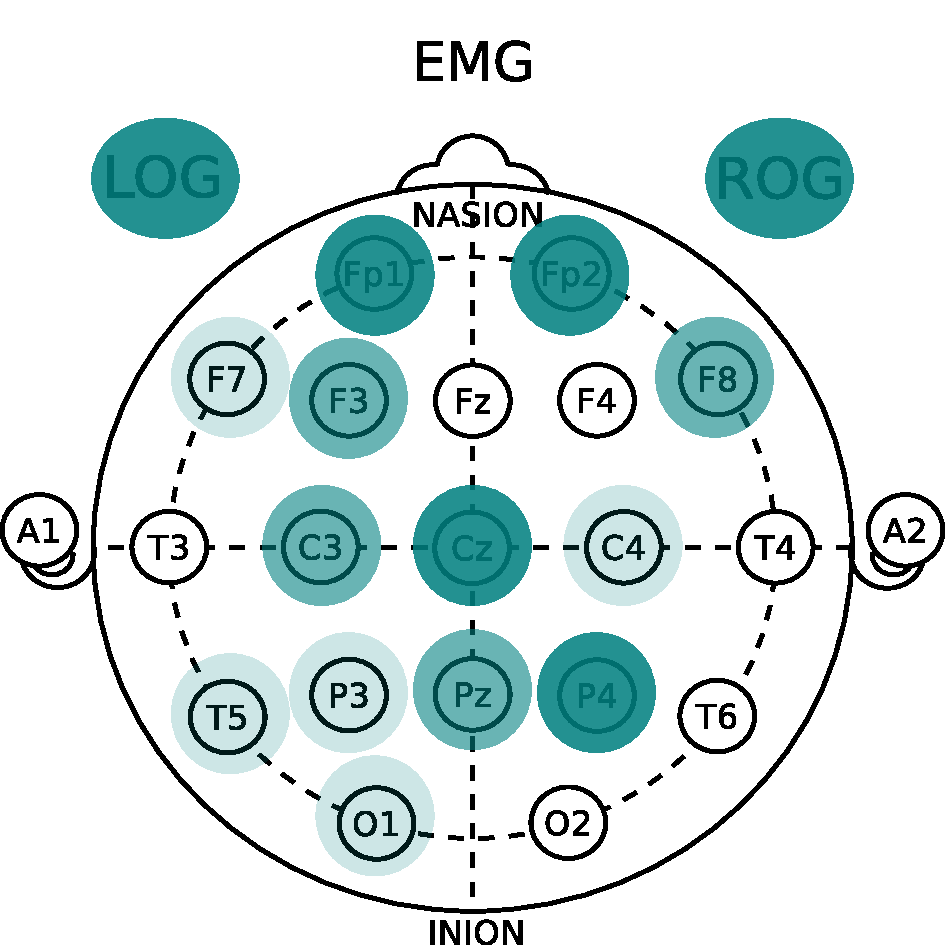
\includegraphics[width=0.17\textwidth]{./img_diagramas/cabecita_VCR.pdf} &
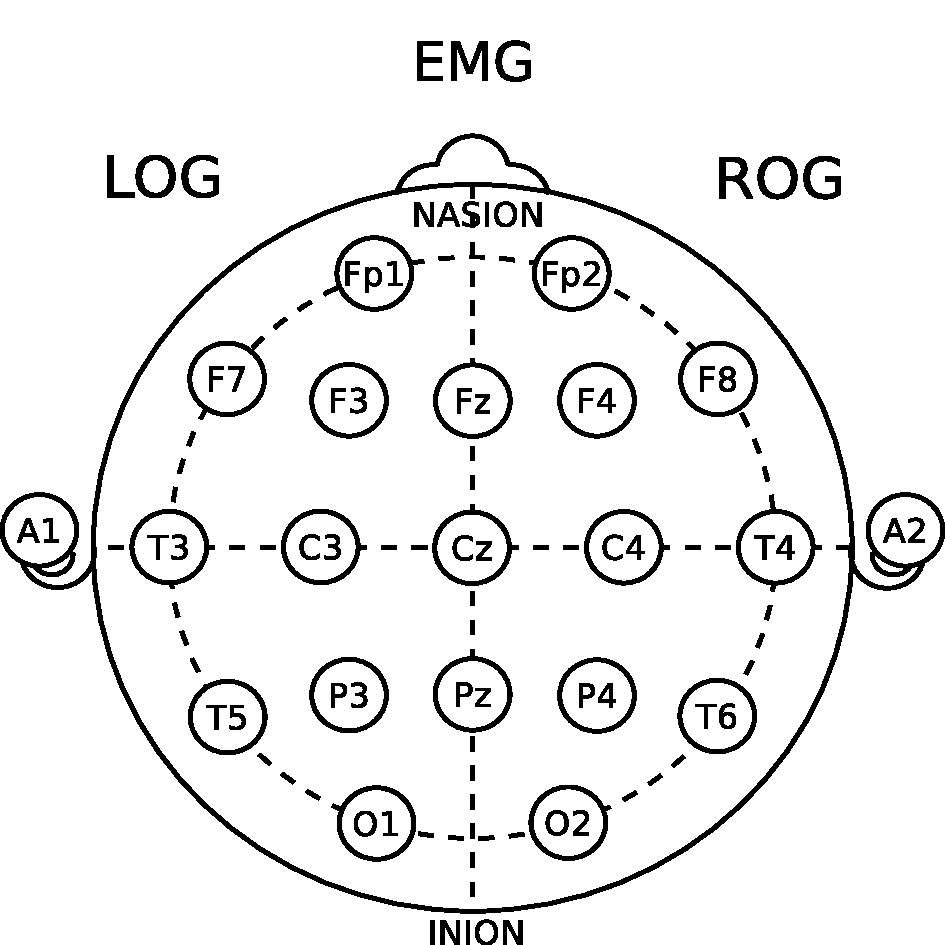
\includegraphics[width=0.17\textwidth]{./img_diagramas/cabecita_MJH.pdf} &
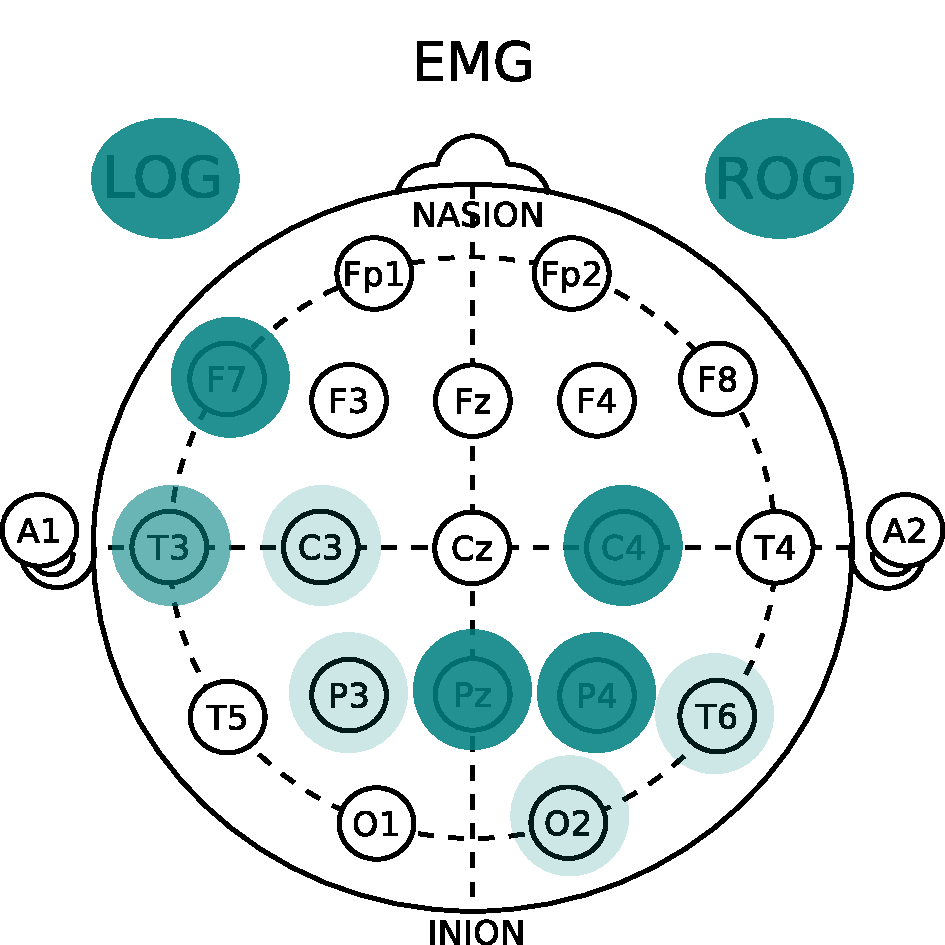
\includegraphics[width=0.17\textwidth]{./img_diagramas/cabecita_JAE.pdf} &
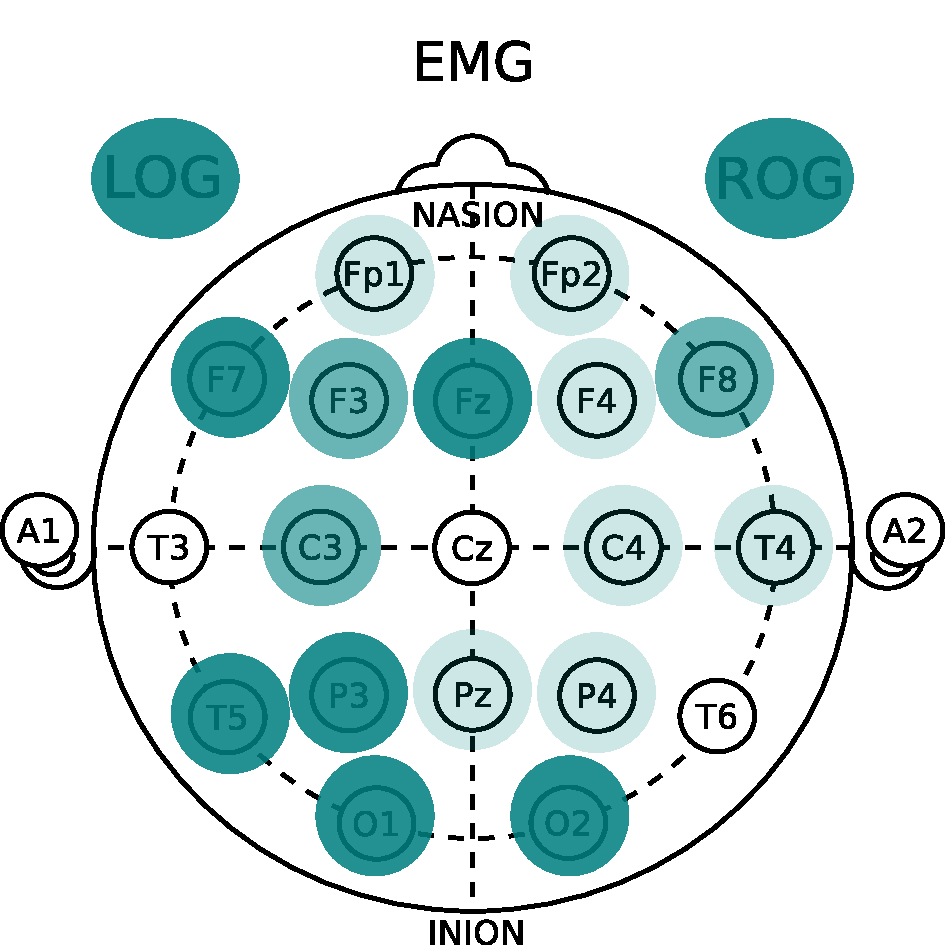
\includegraphics[width=0.17\textwidth]{./img_diagramas/cabecita_GHA.pdf} &
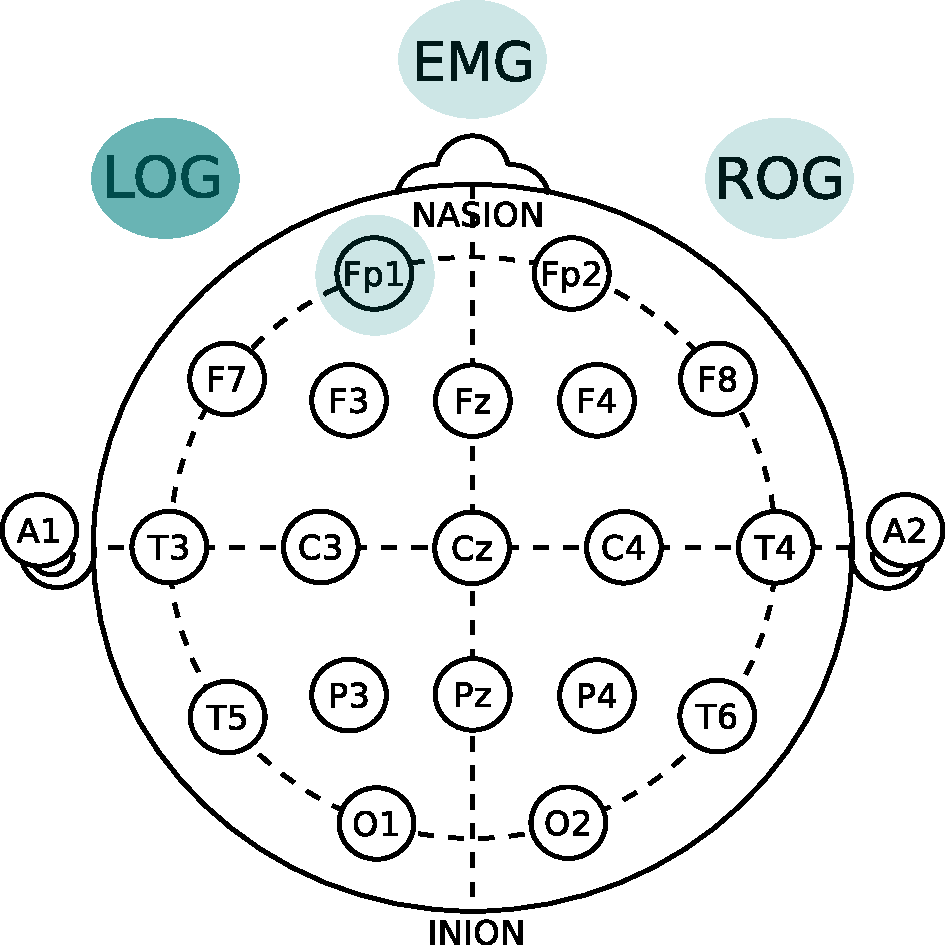
\includegraphics[width=0.17\textwidth]{./img_diagramas/cabecita_MFGR.pdf} \\
VCR & MJH & JAE & GHA & MFGR
\end{tabular}
\\
\begin{tabular}{cccc}
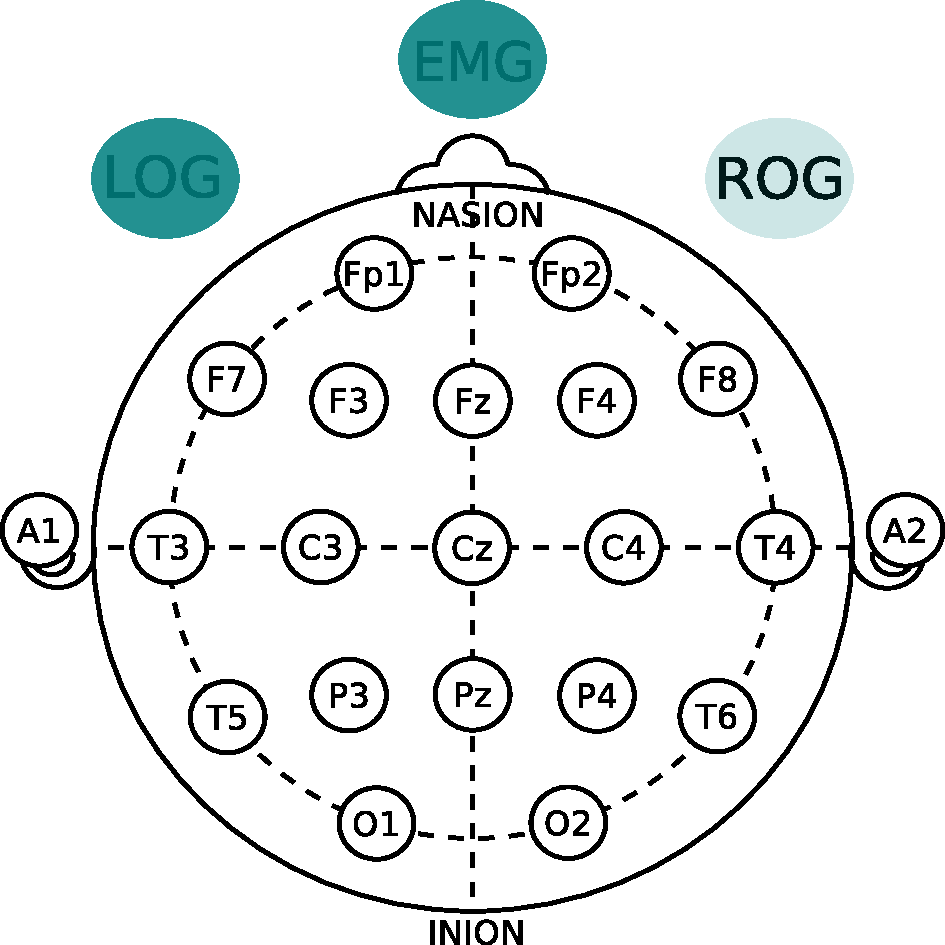
\includegraphics[width=0.17\textwidth]{./img_diagramas/cabecita_CLO.pdf} &
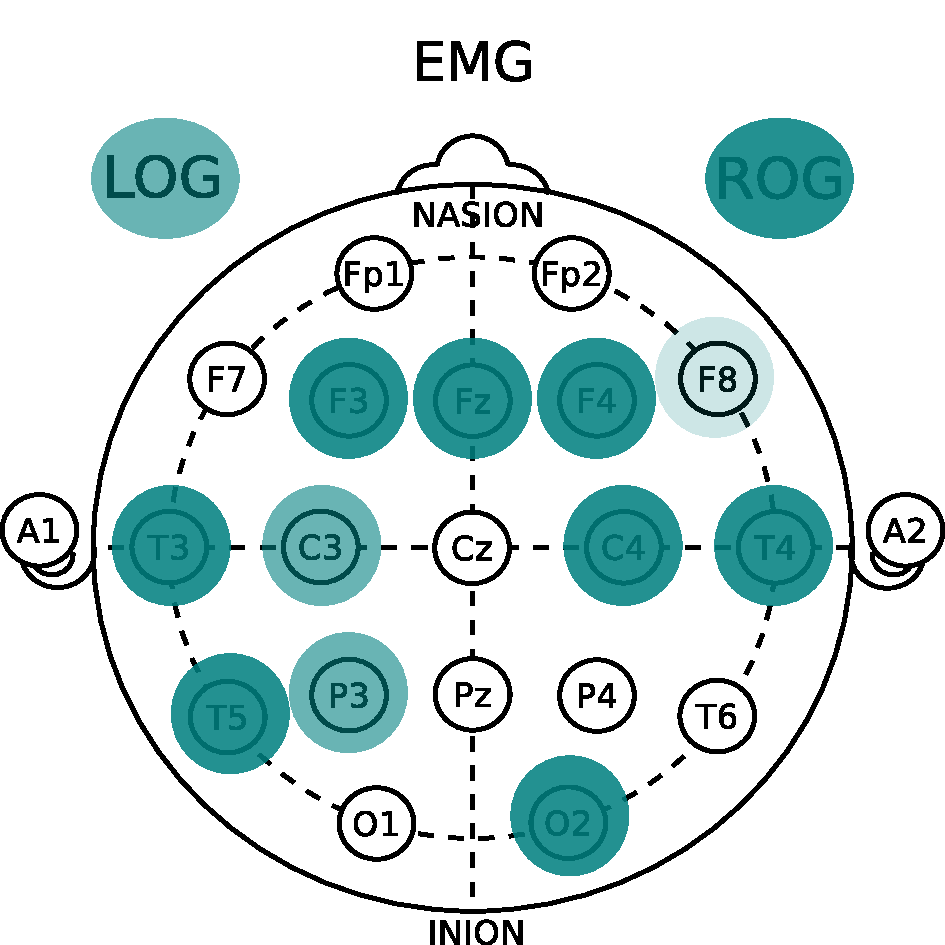
\includegraphics[width=0.17\textwidth]{./img_diagramas/cabecita_RLO.pdf} &
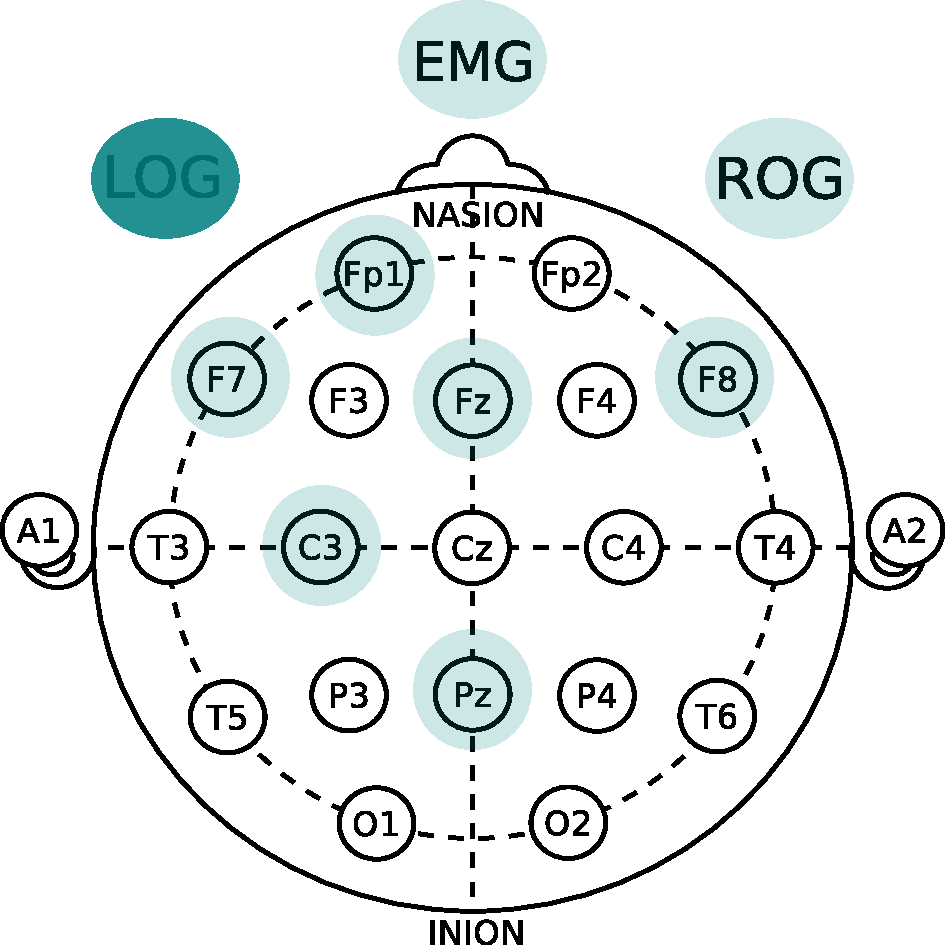
\includegraphics[width=0.17\textwidth]{./img_diagramas/cabecita_RRU.pdf} &
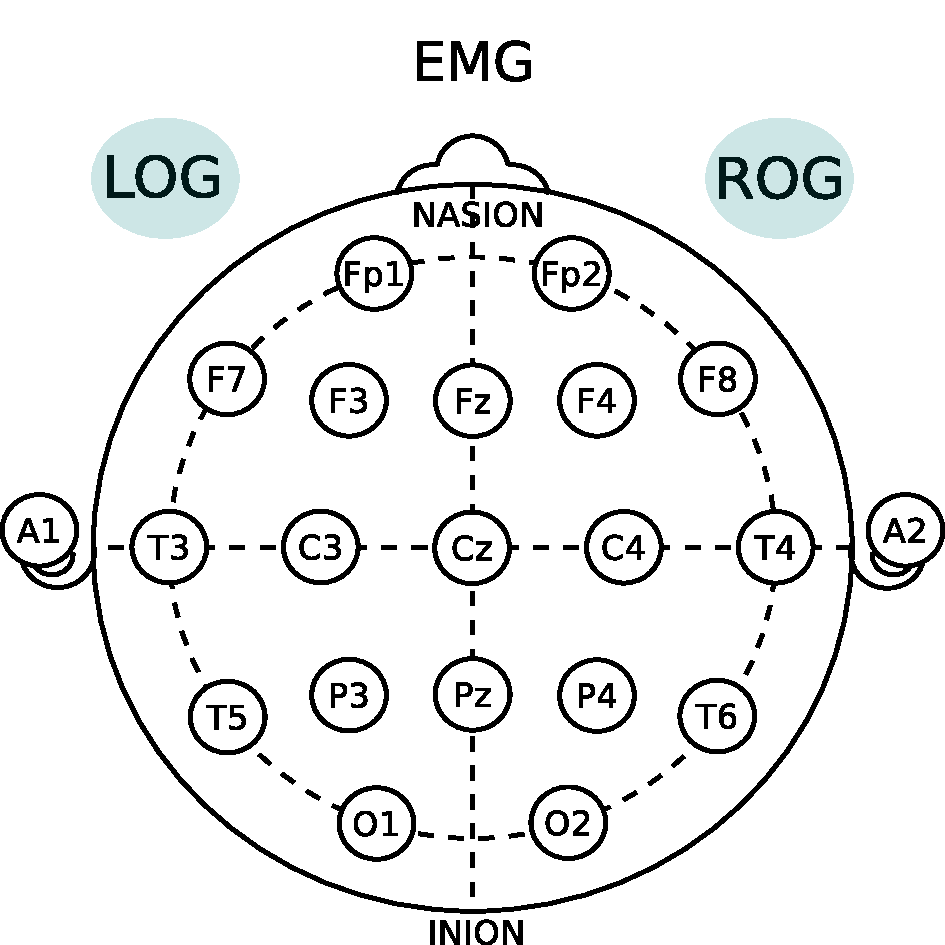
\includegraphics[width=0.17\textwidth]{./img_diagramas/cabecita_JGZ.pdf} \\
CLO & RLO & RRU & JGZ
\end{tabular}
\\
\begin{tabular}{ccc}
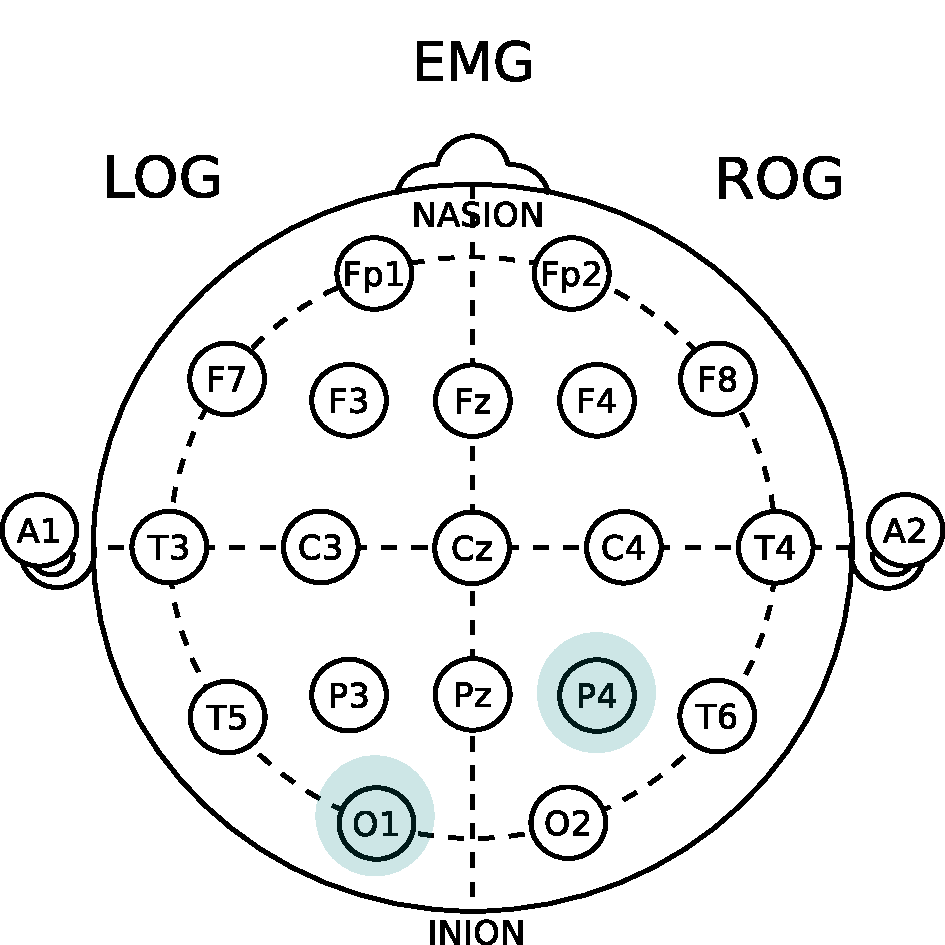
\includegraphics[width=0.17\textwidth]{./img_diagramas/cabecita_FGH.pdf} &
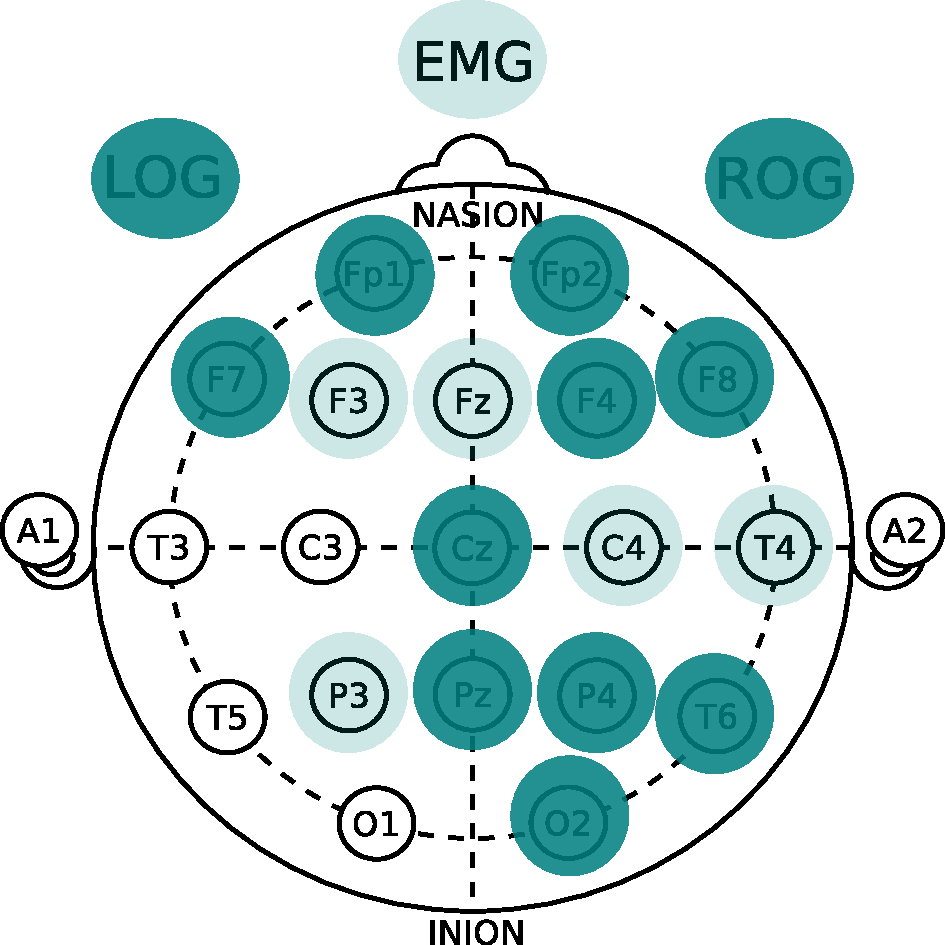
\includegraphics[width=0.17\textwidth]{./img_diagramas/cabecita_MGG.pdf} &
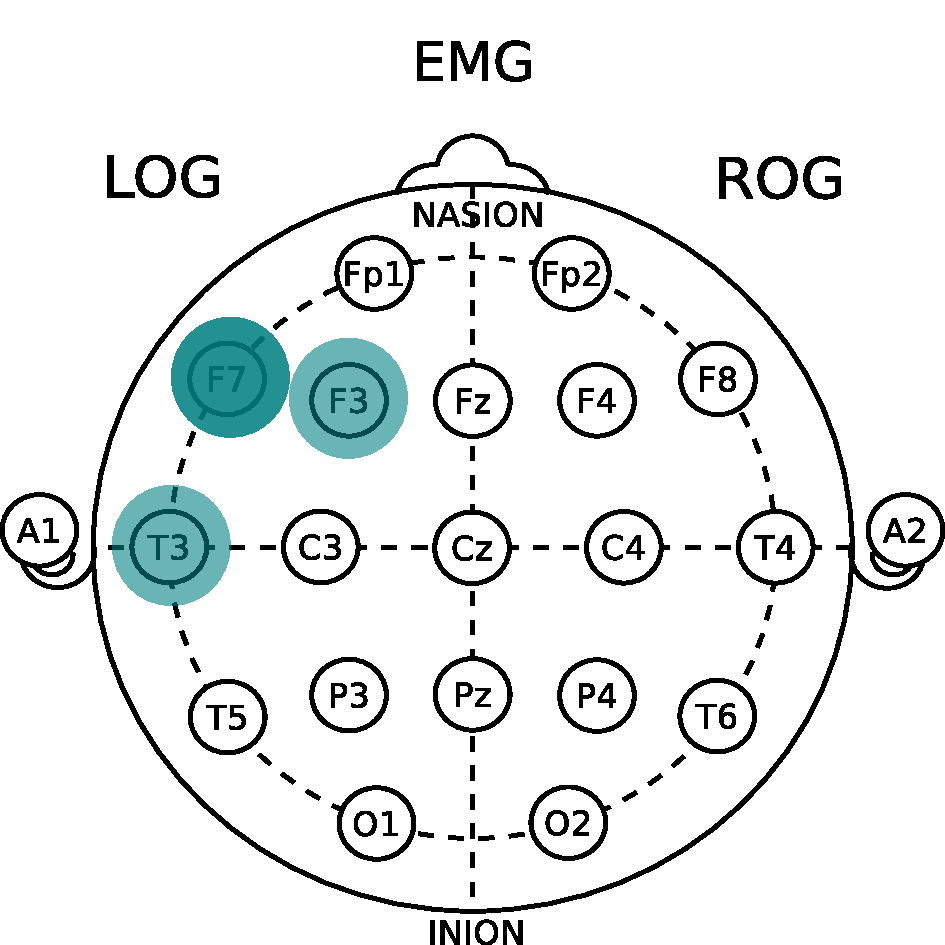
\includegraphics[width=0.17\textwidth]{./img_diagramas/cabecita_EMT.pdf} \\
FGH & MGG & EMT
\end{tabular}
\end{tabular}
\caption{Se muestra esquemáticamente en azul las zonas donde se encontraron diferencias 
significativas al comparar las proporciones de épocas PE durante sueño MOR y NMOR. Esta misma
información se muestra en la tabla \ref{comparacion_mor_vs_total} }
\label{cabecitas_munchas}
\end{figure}

Posteriormente se buscó una diferencia más directa entre los grupos, comparando grupalmente las 
proporciones de épocas PE (en cada canal y durante las diferentes etapas) mediante la prueba U de 
Mann-Whitney\footnote{Implementada en R como la función \texttt{wilcox.test()}}; no se 
encontraron diferencias significativas para ninguno de los canales. Los resultados se muestran en 
las tablas \ref{gpos_mor}, \ref{gpos_nmor}, \ref{gpos_total}, y para una mejor visualización 
éstos se han graficado en la figura \ref{comparacion_graf}.

\begin{figure}
\centering
%\subfloat[Comparación entre épocas MOR (fase R)]{
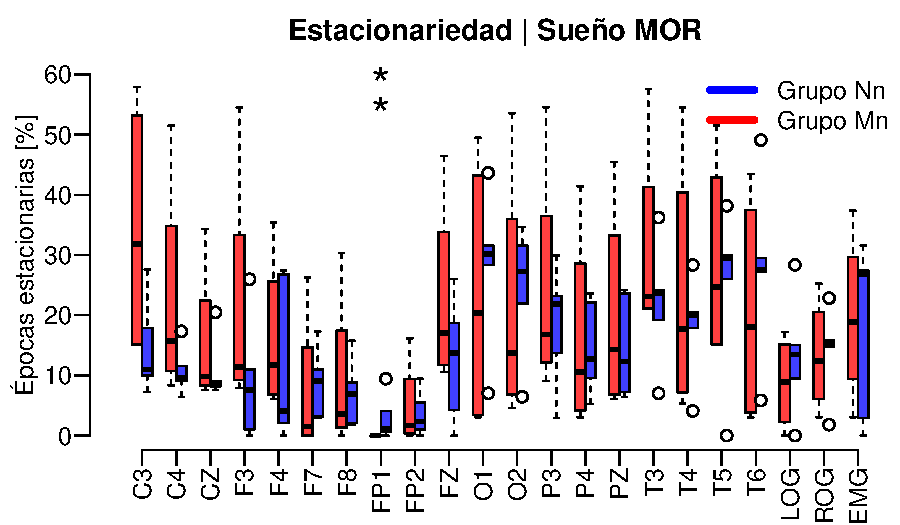
\includegraphics[width=\linewidth]
{./img_ejemplos/Comparacion_gpos_MOR_v2.pdf} \\
%}\\
%\subfloat[Comparación entre épocas no-MOR (fases W y N)]{
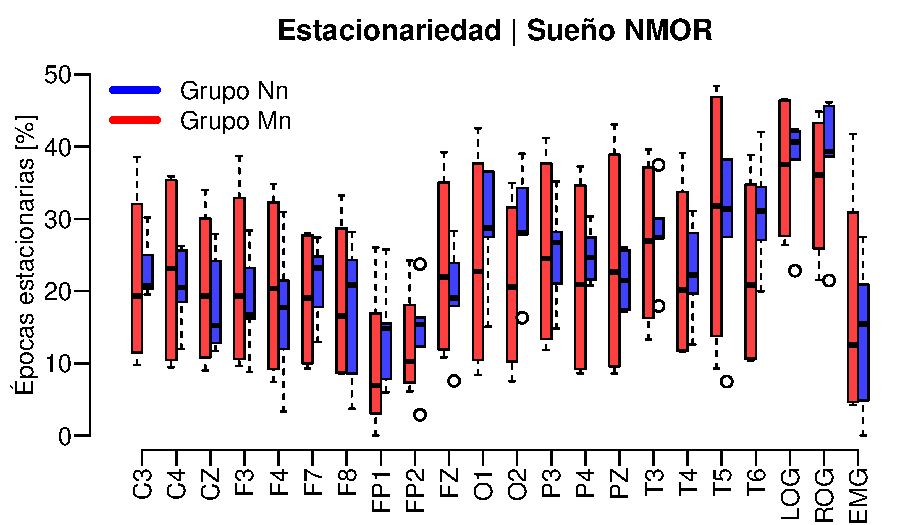
\includegraphics[width=\linewidth]
{./img_ejemplos/Comparacion_gpos_NMOR_v2.pdf}
%}\\
\caption{Comparación sobre las proporciones de épocas estacionarias entre los grupos Nn y Mn, 
durante sueño MOR y NMOR}
\label{comparacion_graf}
\end{figure}

\begin{figure}
\centering
%\subfloat[Comparación para el grupo control]{
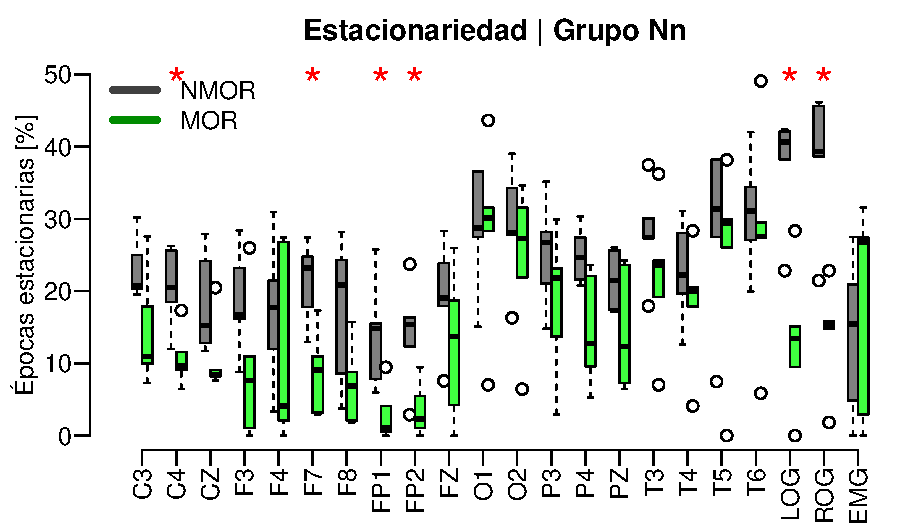
\includegraphics[width=\linewidth]
{./img_ejemplos/Comparacion_etapas_normal_MOR_vs_NMOR_v2.pdf} \\
%}\\
%\subfloat[Comparación para el grupo PDC]{
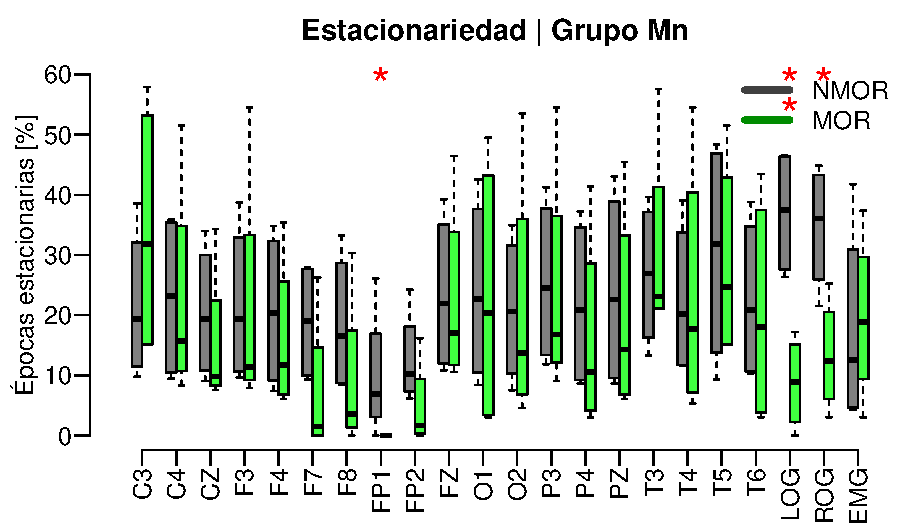
\includegraphics[width=0.95\linewidth]
{./img_ejemplos/Comparacion_etapas_pdc_MOR_vs_NMOR_v2.pdf} \\
%}
\caption{Comparación sobre las proporciones de épocas estacionarias durante sueño MOR y NMOR, para 
ambos grupos}
\label{comparacion_verde}
\end{figure}

Una segunda variación del primer análisis es considerar grupalmente a los sujetos como 
'unidades' que transitan entre etapas de sueño; se comparan grupalmente las proporciones de 
épocas PE en cada canal durante sueño MOR y NMOR, usando la prueba U de Mann-Whithney; en 
la figura \ref{comparacion_verde} se han representado gráficamente estas diferencias.
Se encontró que hay diferencias significativas ($\alpha<0.05$) para el grupo Control en los 
canales C3, C4, F7, F8, FP1, FP2, O2, P4, LOG y ROG, mientras que en el grupo PDC sólo se
observaron diferencias en LOG y ROG.
Descartando los canales LOG y ROG, ya que no son parte del EEG, las diferencias encontradas pueden 
ser relevantes fisiológicamente, ya que abarcan gran parte de los lóbulos frontal y parietal, 
y parte de la región occipital-parietal derecha; en la figura \ref{cabecita} se indican 
esquemáticamente estas regiones.

%\begin{figure}
%\centering
%\includegraphics[width=0.4\linewidth]
%{./img_diagramas/cabecita.pdf} 
%\caption{Representación esquemática de los sitios donde se encontraron diferencias 
%significativas en la comparación entre el porcentaje de épocas PE durante sueño MOR y NMOR, 
%para el grupo Control (ver texto)}
%\label{cabecita}
%\end{figure}

%%%%%%%%%%%%%%%%%%%%%%%%%%%%%%%%%%%%%%%%%%%%%%%%%%%%%%%%%%%%%%%%%%%%%%%%%%%%%%%%%%%%%%%%%%%%%%%%%%%
%%%%%%%%%%%%%%%%%%%%%%%%%%%%%%%%%%%%%%%%%%%%%%%%%%%%%%%%%%%%%%%%%%%%%%%%%%%%%%%%%%%%%%%%%%%%%%%%%%%

\section{Patrones visuales}

Como un análisis exploratorio, buscando explicar la variabilidad entre los resultados, se 
graficaron los resultados obtenidos con la prueba PSR de la siguiente manera: se colocan en 
línea horizontal una serie de cuadros, uno por cada época analizada según fue clasificada 
(blanco: PE, negro: no-estacionario), y posteriormente se juntaron verticalmente las líneas
correspondientes a los diferentes canales; en la figura \ref{ejemplo_graf} se muestra un ejemplo de
ello, mientras que en el anexo se muestran los gráficos construidos para cada uno de los sujetos. 

Al construir estos gráficos, se hacen presentes 'bloques' de épocas que en su mayoría son
PE --similarmente con épocas no-estacionarias. Ha parecido conveniente reportar este hallazgo
ya que los patrones son consistentes en todos los sujetos, y porque parece que estos 'bloques'
aparecen asociados al sueño MOR en cierto orden (ilustrado en la figura \ref{patroncito}):
\begin{itemize}
\item Bloque abundante en épocas PE, visualmente oscuro
\item Bloque abundante en épocas no-estacionarias, visualmente claro
\item Sección que contiene el sueño MOR, los canales LOG y ROG muestran son visualmente más
abundante en épocas no-estacionarias en esta zona del tiempo
\end{itemize}

\begin{figure}
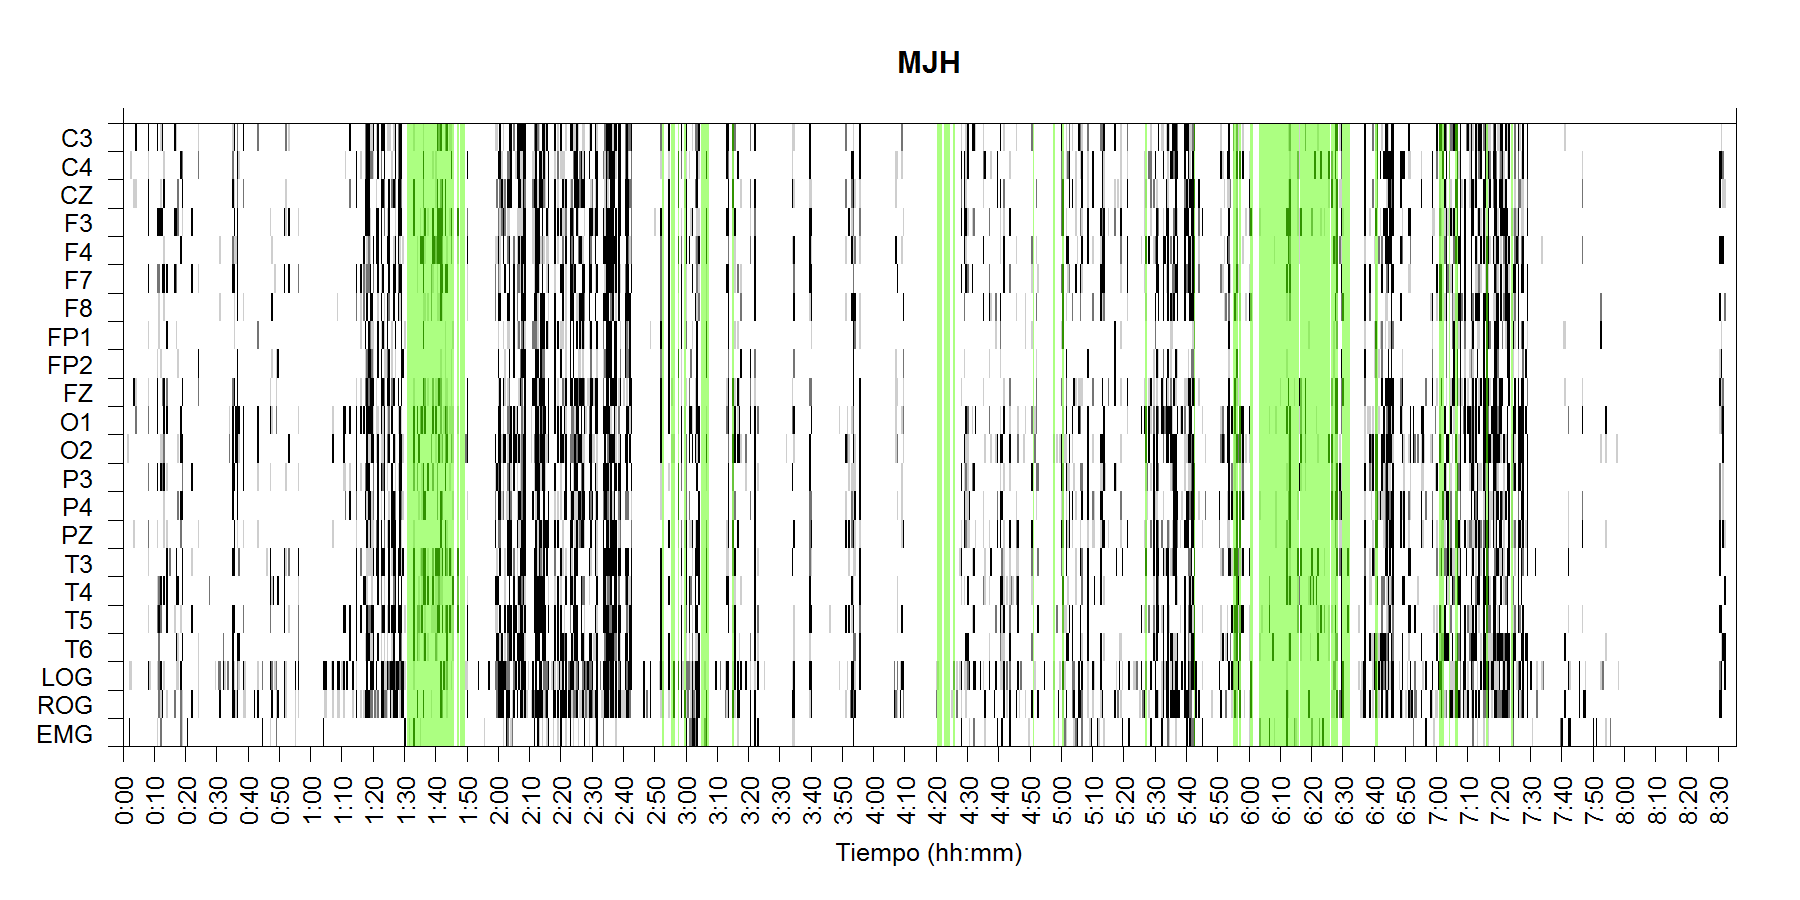
\includegraphics[width=\textwidth]
{./img_ejemplos/MJNNVIGILOS_est.png}
\caption{Disposición gráfica para los resultados de la prueba PSR en el sujeto MJH. Se han 
resaltado con color verde las épocas clasificadas como de sueño MOR.}
\label{ejemplo_graf}
\end{figure}

\begin{figure}
\begin{tabular}{c}
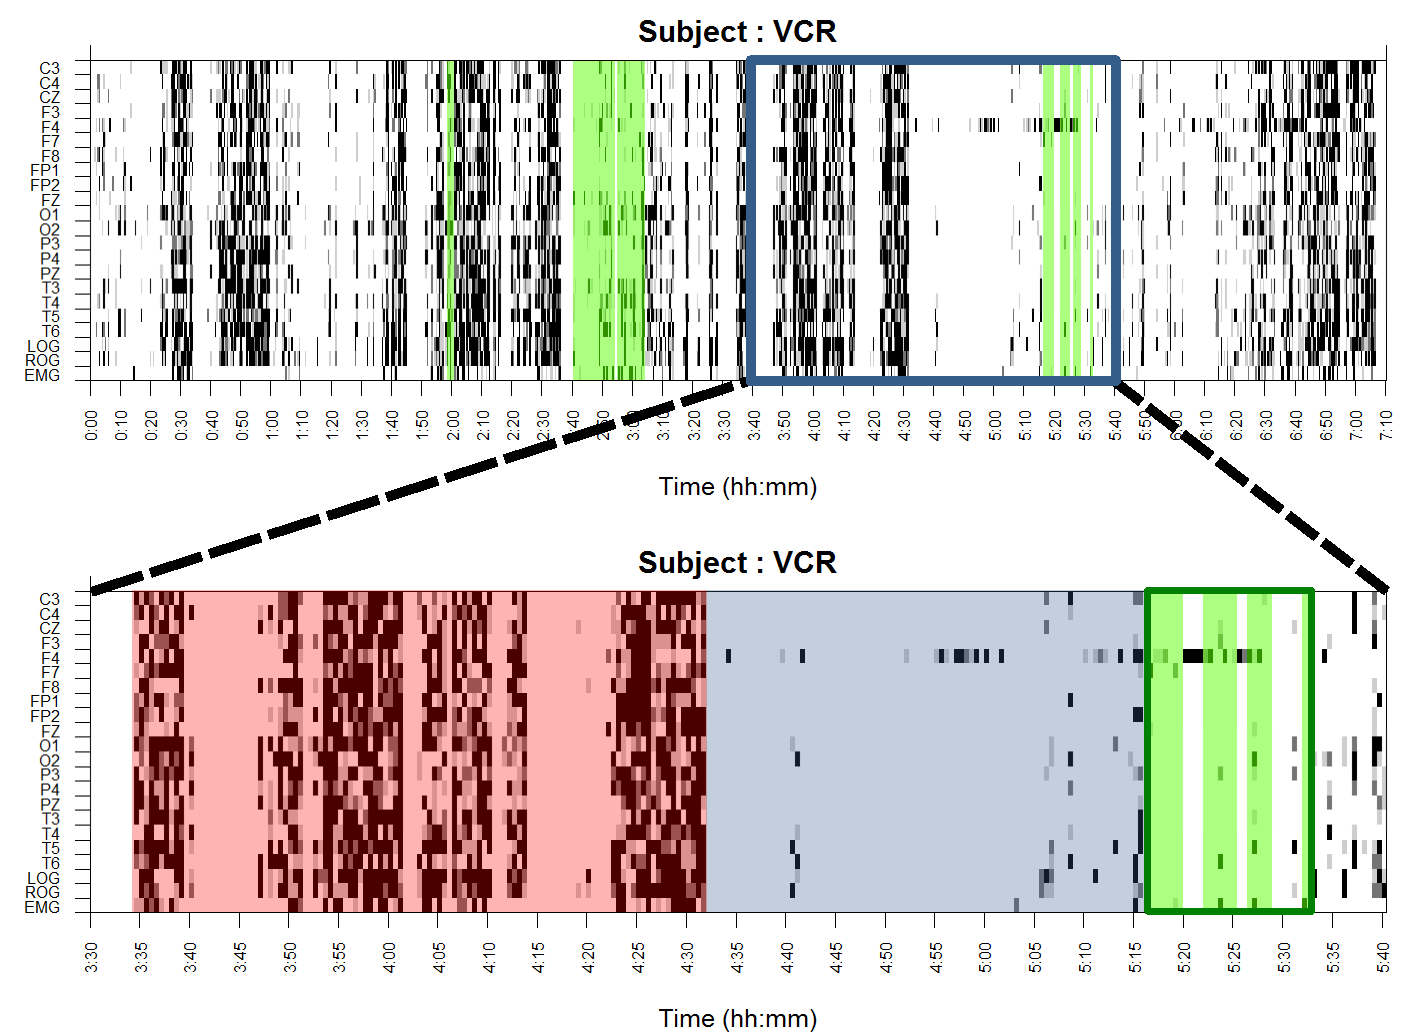
\includegraphics[width=0.3\textwidth]
{./img_ejemplos/zoom_VCR.pdf}
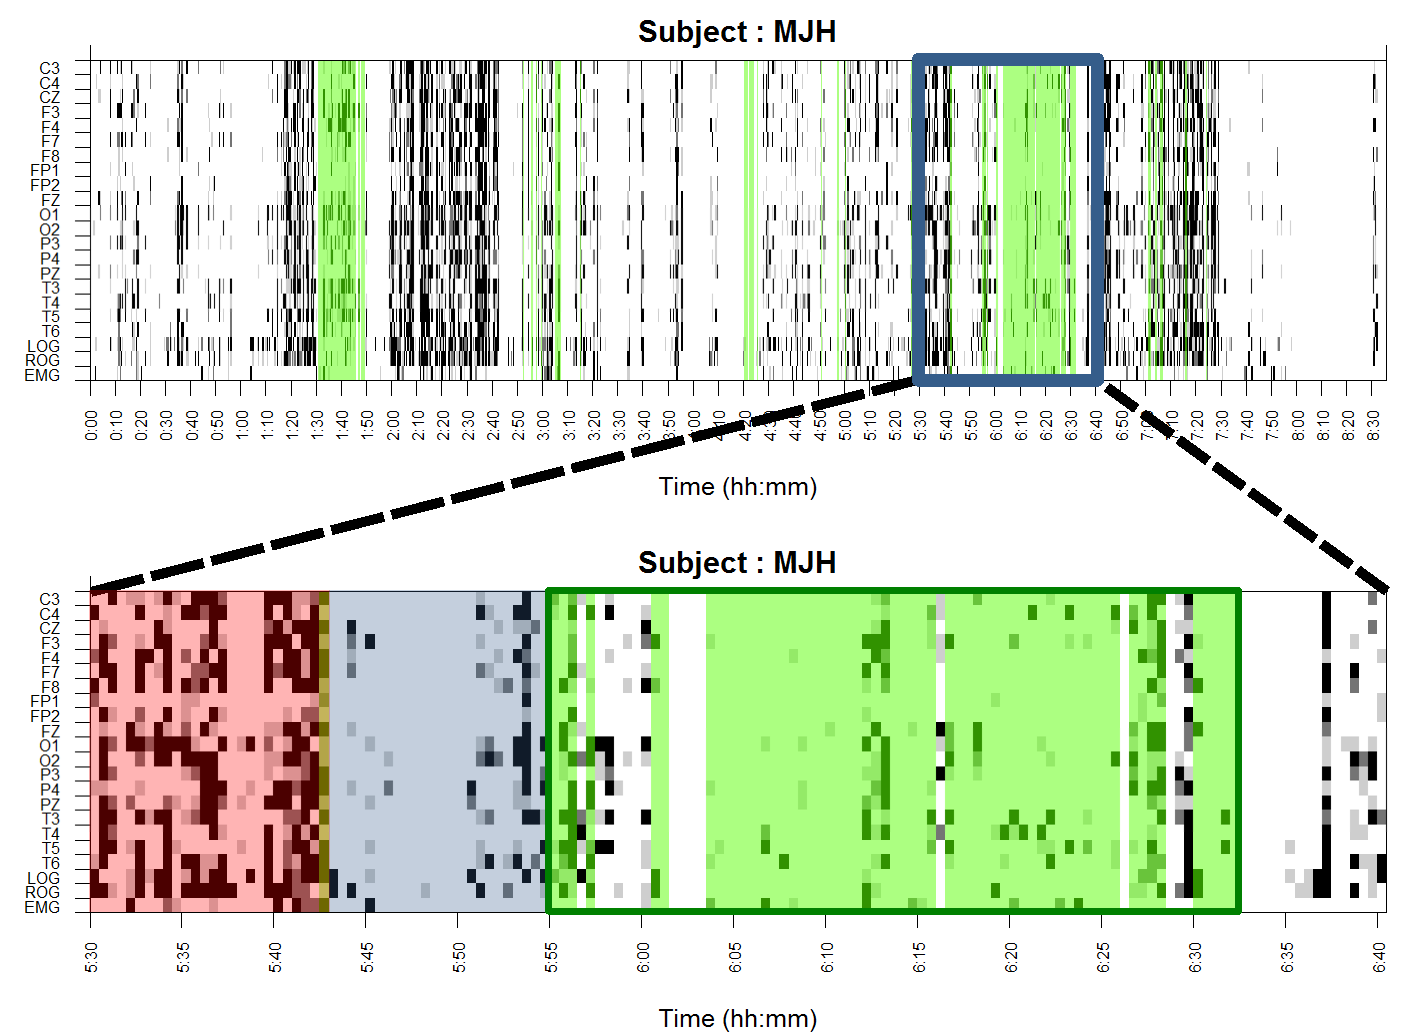
\includegraphics[width=0.3\textwidth]
{./img_ejemplos/zoom_MJH.pdf}
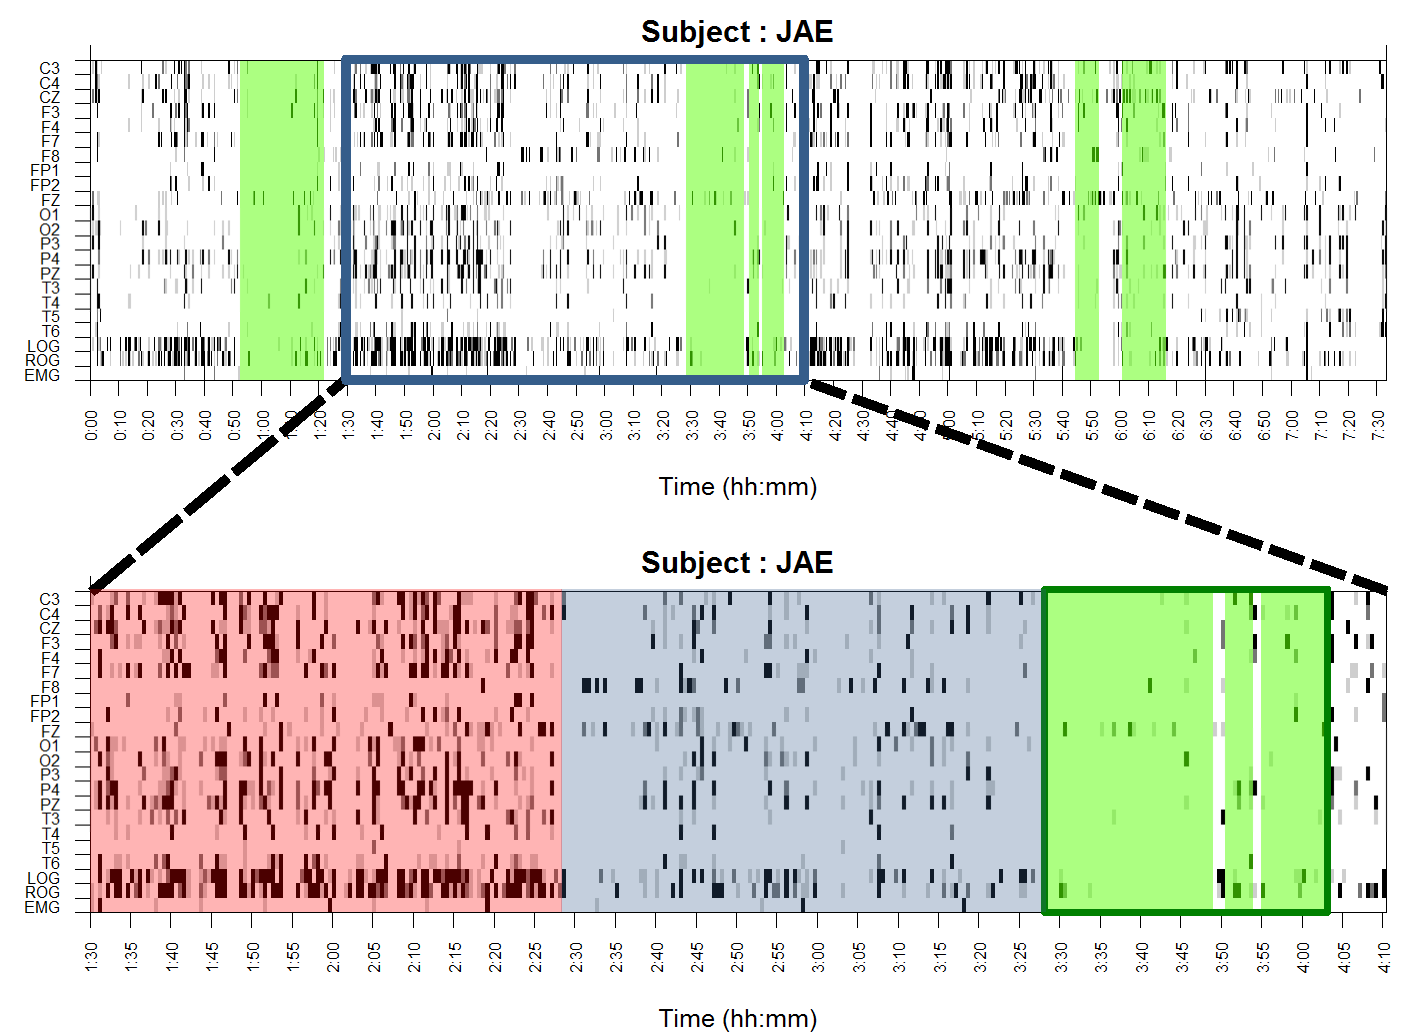
\includegraphics[width=0.3\textwidth]
{./img_ejemplos/zoom_JAE.pdf}
\\
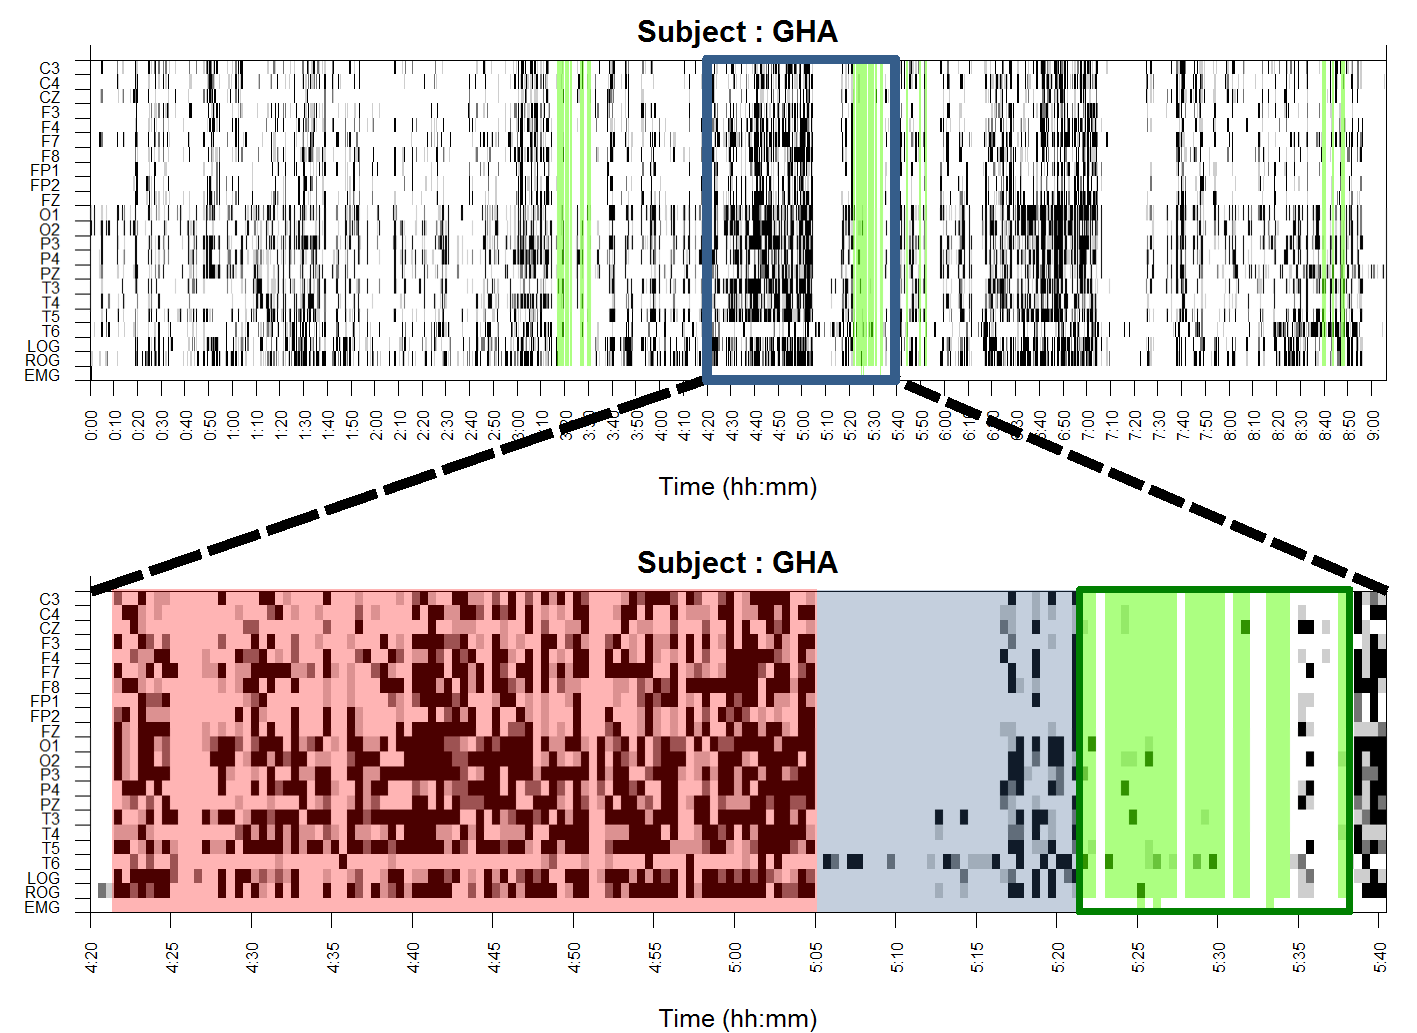
\includegraphics[width=0.3\textwidth]
{./img_ejemplos/zoom_GHA.pdf}
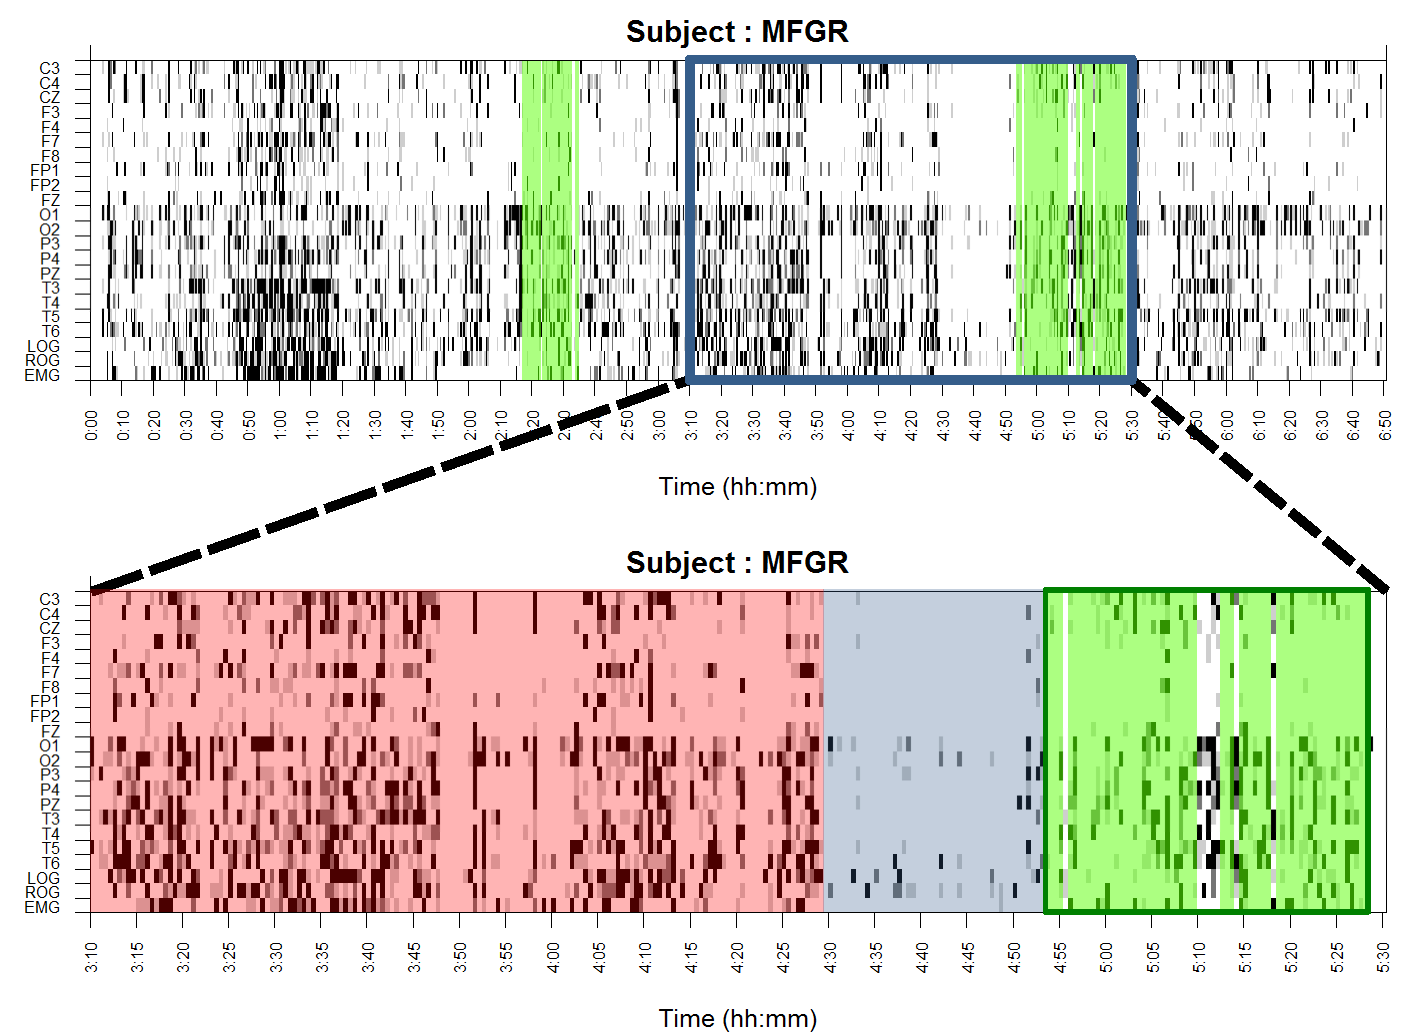
\includegraphics[width=0.3\textwidth]
{./img_ejemplos/zoom_MFGR.pdf}
\end{tabular}
\caption{Ejemplos de los patrones visuales que, se propone, está asociado con la aparición del
sueño MOR: un bloque de épocas PE (rojo), un bloque de épocas no-estacionarias (azul) y un 
bloque que contiene al sueño MOR. En este ejemplo se ilustra uno de estos patrones por cada
uno de los sujetos del grupo Control.}
\label{patroncito}
\end{figure}

%%%%%%%%%%%%%%%%%%%%%%%%%%%%%%%%%%%%%%%%%%%%%%%%%%%%%%%%%%%%%%%%%%%%%%%%%%%%%%%%%%%%%%%%%%%%%%%%%%%
%%%%%%%%%%%%%%%%%%%%%%%%%%%%%%%%%%%%%%%%%%%%%%%%%%%%%%%%%%%%%%%%%%%%%%%%%%%%%%%%%%%%%%%%%%%%%%%%%%%
%%%%%%%%%%%%%%%%%%%%%%%%%%%%%%%%%%%%%%%%%%%%%%%%%%%%%%%%%%%%%%%%%%%%%%%%%%%%%%%%%%%%%%%%%%%%%%%%%%%
%%%%%%%%%%%%%%%%%%%%%%%%%%%%%%%%%%%%%%%%%%%%%%%%%%%%%%%%%%%%%%%%%%%%%%%%%%%%%%%%%%%%%%%%%%%%%%%%%%%

\section{Discusión}

Como se mencionó anteriormente, este trabajo parte del supuesto en que los sujetos con PDC 
presentan con mayor probabilidad estacionariedad débil en sus registros de EEG.
Se ha aportado evidencia para afirmar que, al comparar sujetos del grupo Control y con PDC, no hay 
cambios significativos en la porción de tiempo durante la cual el registro de PSG se comporta 
como débilmente estacionario. 
Esto puede interpretarse como que, quizá, los mecanismos afectados durante el PDC no provocan que 
la señal se vuelva más 'simple' (en el sentido de ser estacionaria).

Cabe un comentario sobre cómo la evidencia presentada exhibe al PSG como un conjunto de señales 
no-estacionarias durante la mayor parte del sueño, como se suele suponer en señales de origen 
biológico; entonces, no es adecuado analizar este tipo de señales con métodos que supongan 
estacionariedad, como la estimación del espectro de potencias usando el periodograma 'clásico'. 

%%%%%%%%%%%%%%%%%%%%%%%%%%%%%%%%%%%%%%%%%%%%%%%%%%%%%%%%%%%%%%%%%%%%%%%%%%%%%%%%%%%%%%%%%%%%%%%%%%%
%%%%%%%%%%%%%%%%%%%%%%%%%%%%%%%%%%%%%%%%%%%%%%%%%%%%%%%%%%%%%%%%%%%%%%%%%%%%%%%%%%%%%%%%%%%%%%%%%%%

\subsection{Sobre los sujetos excluidos}

Durante el trabajo se mencionan tres sujetos (FGH, MGG, EMT) cuyos registros de PSG fueron 
analizados pero que no son considerados estadísticamente; cada uno de ellos fue excluido, por 
diversos motivos, del trabajo por Vázquez Tagle y colaboradores \cite{VazquezTagle16}, pero 
dieron su consentimiento informado para el registro de PSG, debido a lo cual analizó el efecto de 
su inclusión dentro de los análisis.
Destaca el sujeto FGH, quien padece de parálisis facial, cataratas, y problemas no especificados 
en hipotiroides y columna; según se reporta, el sujeto no informó de estos últimos 
padecimientos sino hasta después del registro de PSG, por lo que su exclusión se efectuó a 
posteriori.

Un vistazo a los registros 'inusuales' de FGH (figura\ref{FGH_psg}, comparar con 
\ref{ejemplos_mor}) pudiera haber advertido que en el registro no hay actividad cerebral en los 
canales correspondientes a la región izquierda (aquella con parálisis) sino ruido amplificado 
del polisomnógrafo.
Dentro del marco de este trabajo, destacan las proporciones inusuales de épocas PE (cercanas a 1 
o 0) para este sujeto en los canales F4, F7, F8, FP1, FP2, FZ, tanto en sueño MOR como NMOR; 
usando la representación gráfica para FGH, es visible una inusual ausencia total de 
estacionariedad en tales canales (figura \ref{FGH_especial}, comparar con \ref{ejemplo_graf}). 
Si bien esta metodología no se diseñó para tal fin, aún así se pudo detectar la falta de 
actividad cerebral.

\begin{figure}
\centering
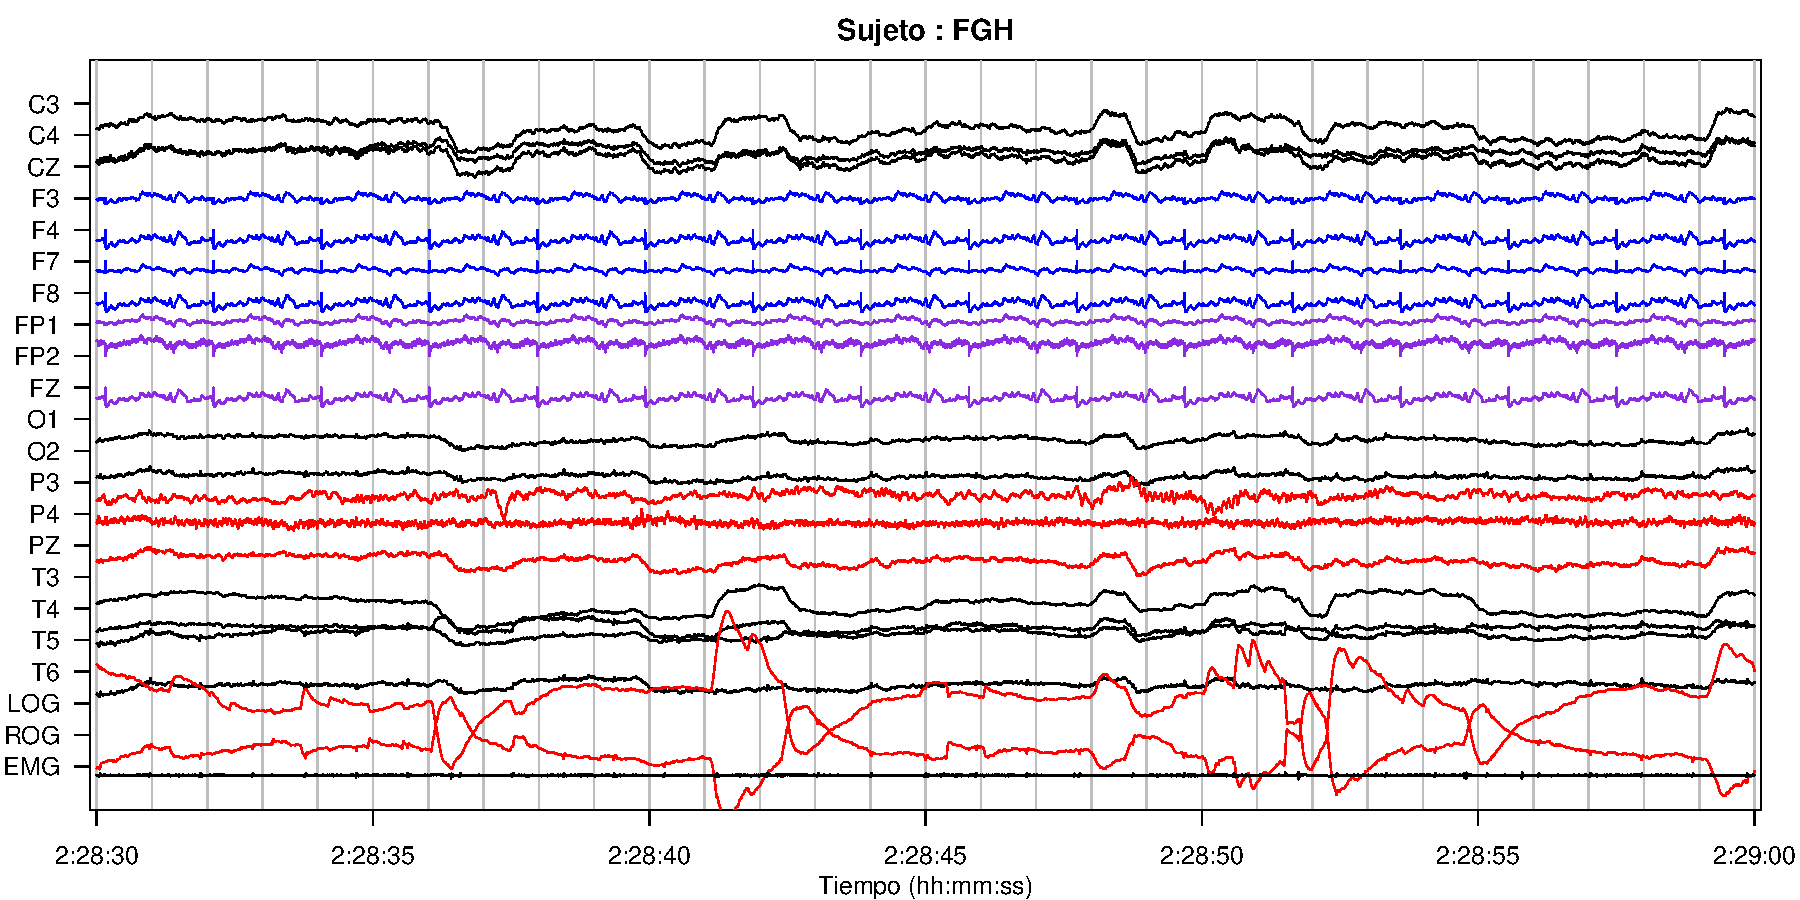
\includegraphics[width=0.95\linewidth]
{./img_ejemplos/FGH_297_PDG_lucirse_PSG.pdf} 
\caption{Una época típica del registro PSG para el sujeto FGH durante sueño MOR. Nótense 
los patrones periódicos en los canales correspondientes a la región frontal, que no 
corresponden a la actividad cerebral usual.}
\label{FGH_psg}
\end{figure}

\begin{figure}
\centering
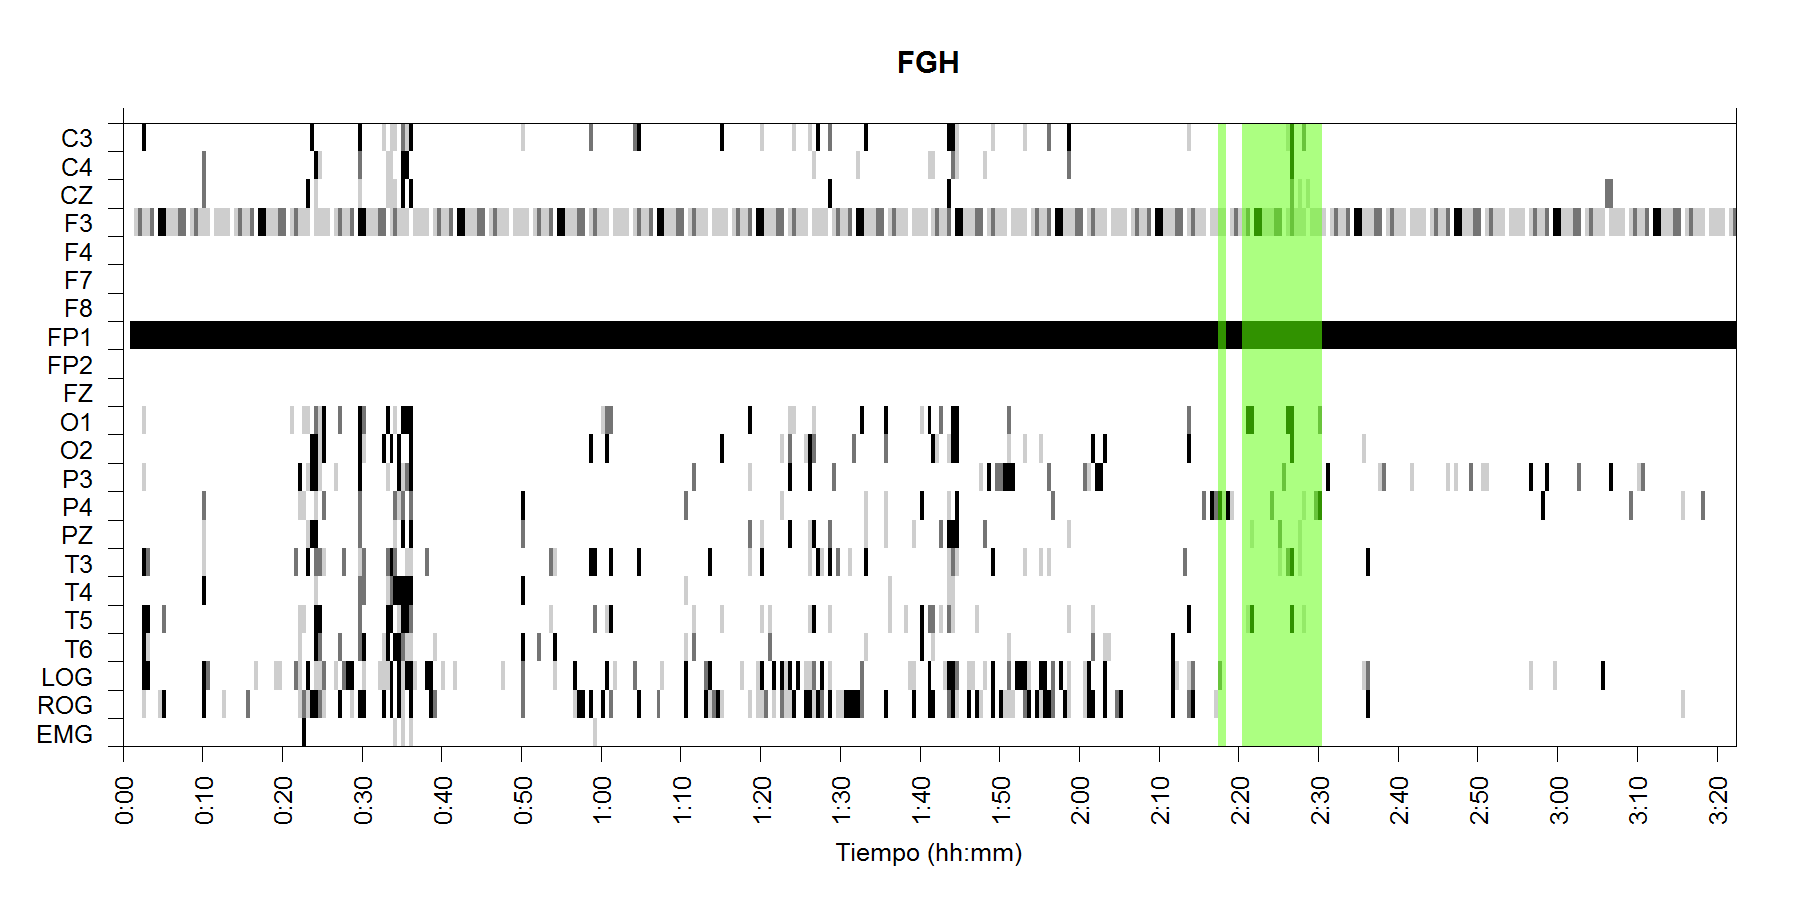
\includegraphics[width=0.95\linewidth]
{./img_ejemplos/FGHSUE_est.png} 
\caption{Compilado gráfico para el sujeto FGH; nótese el patrón inusual (completamente 
blanco o negro) en los canales correspondientes a la región frontal}
\label{FGH_especial}
\end{figure}

%%%%%%%%%%%%%%%%%%%%%%%%%%%%%%%%%%%%%%%%%%%%%%%%%%%%%%%%%%%%%%%%%%%%%%%%%%%%%%%%%%%%%%%%%%%%%%%%%%%
%%%%%%%%%%%%%%%%%%%%%%%%%%%%%%%%%%%%%%%%%%%%%%%%%%%%%%%%%%%%%%%%%%%%%%%%%%%%%%%%%%%%%%%%%%%%%%%%%%%

\subsection{Efecto del tamaño de las época}

El uso de épocas de 30 segundos está motivado por las recomendaciones de la AASM para 
clasificar, de manera estandarizada, las etapas de sueño a partir de registros de PSG 
\cite{AASM07}. 
No se discutirán en este trabajo motivaciones o evidencia para usar esta longitud de época en 
particular, ni para el caso contrario, sino que se acepta por fines de comparabilidad. 
Sin embargo, en algún momento de este trabajo se usaron los registros de PSG organizados en 
épocas de 10 segundos de duración, como se muestra en la figura \ref{epocas_diferentes}. 
Se realizaron todos los análisis descritos usando esta segmentación mixta (algunos sujetos con 
épocas de 10 s, otros con épocas de 30 s) y se obtuvieron resultados según los cuales no hay 
diferencias significativas en ninguno de los análisis. 
Por otro lado, la representación gráfica construida a partir de los mismos datos, organizados
en épocas de 10 s, cambia sustancialmente (ver figura \ref{comp_VCR}).

\begin{figure}
\centering
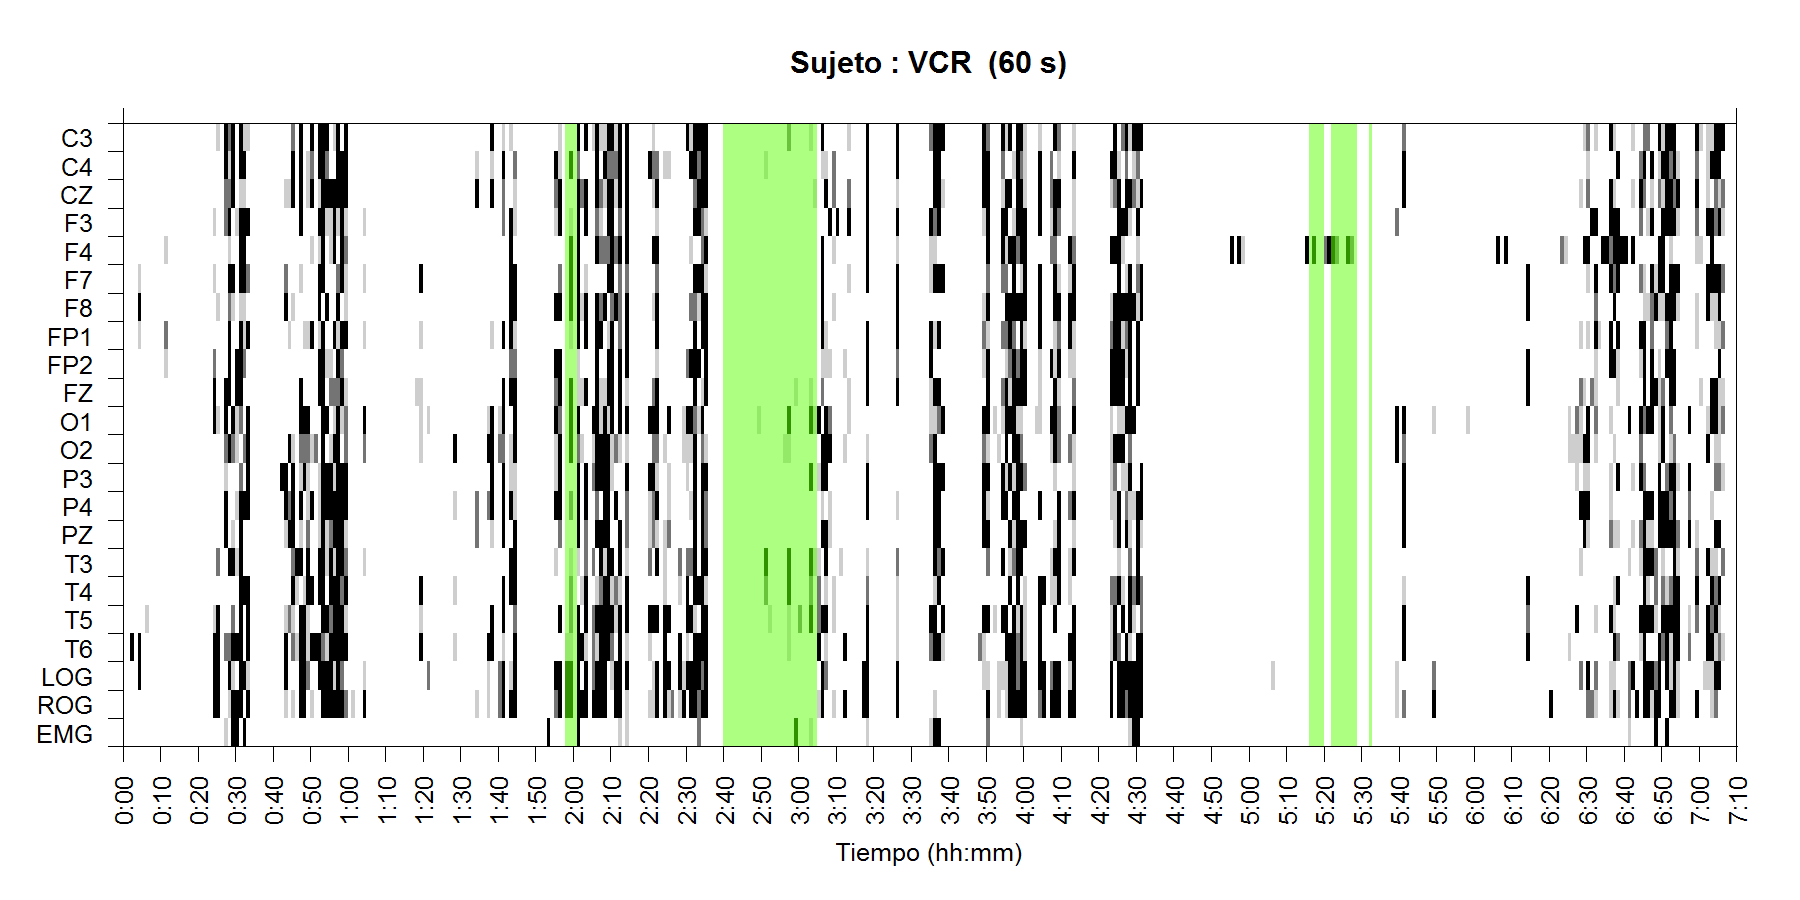
\includegraphics[width=0.9\linewidth] 
{./img_ejemplos/VCNNS1_est_60.png} 
\\
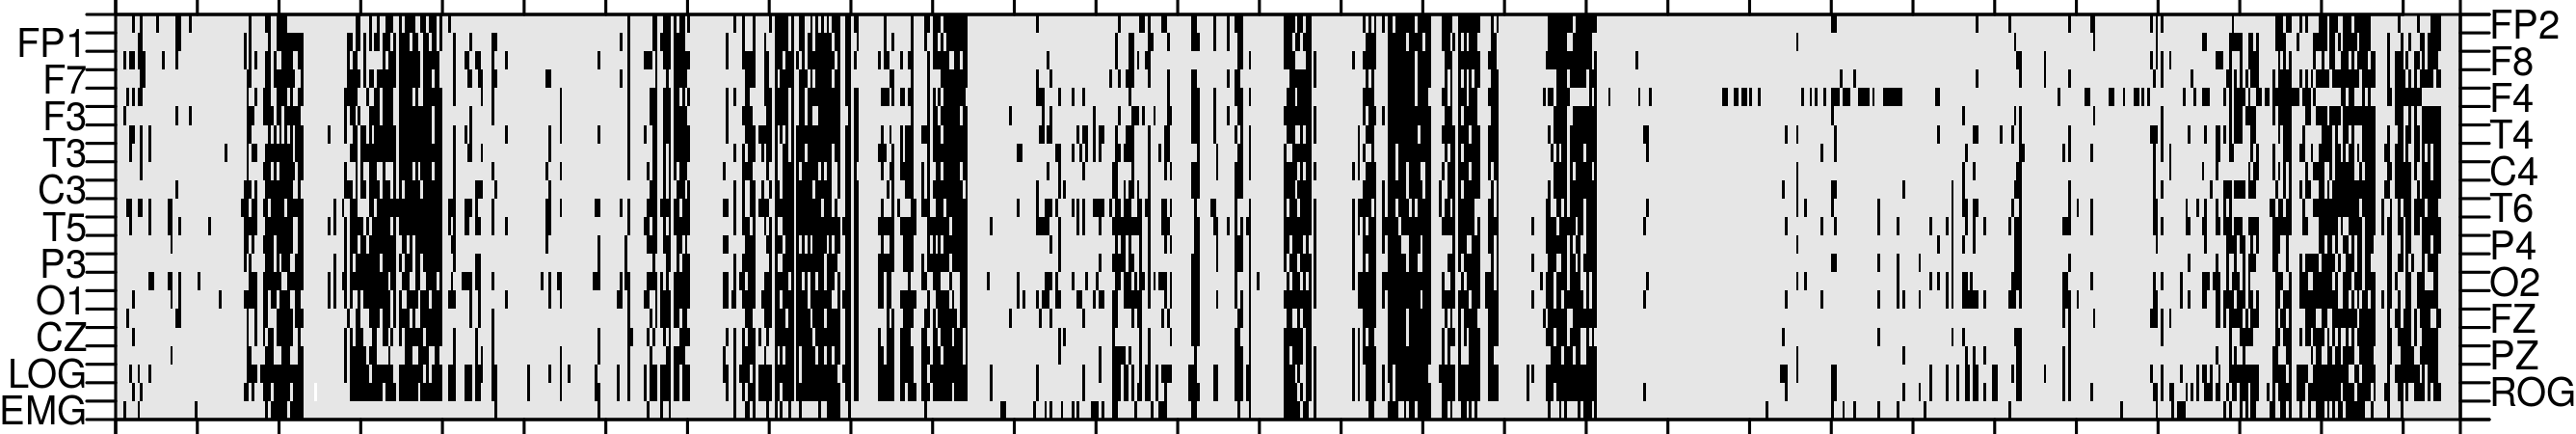
\includegraphics[width=0.9\linewidth]
{./img_ejemplos/VCNNS1_est_30.png} 
\\
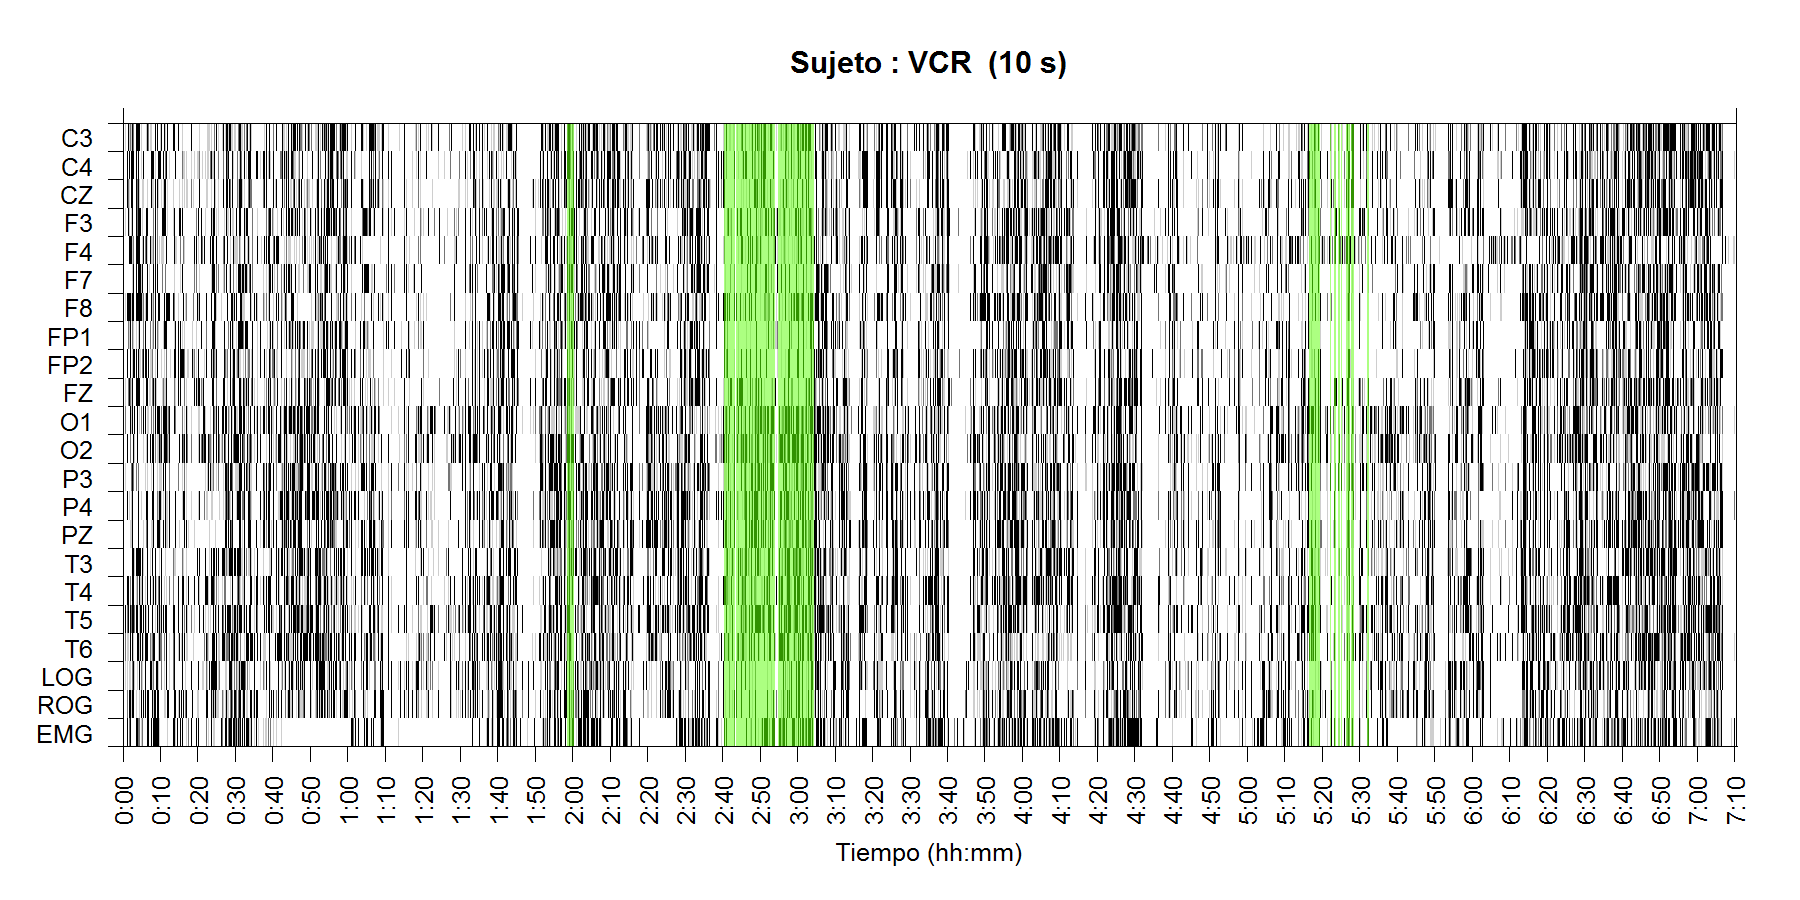
\includegraphics[width=0.9\linewidth]
{./img_ejemplos/VCNNS1_est_10.png} 
\caption{Compilación gráfica de las épocas clasificadas como PE, distribuidas en el tiempo
para cada uno de los canales. El registro corresponde al sujeto VCR, organizando el registro en
épocas de diferente duración}
\label{comp_VCR}
\end{figure}

El hecho de que los resultados fueran afectados de manera contundente por la forma en que se 
organizan los datos, sugiere que será provechoso prestar mayor atención a la naturaleza de las 
características estudiadas y su posible interpretación en la fisiología.
Se propone que los registros de PSG tienen una propiedad referida como 'estacionariedad local',
concepto introducido por Dahlhaus \cite{Dahlhaus97}.
A grosso modo, un proceso localmente estacionario es aquél cuya FDE (que puede depender del 
tiempo) puede ser aproximada 'a trozos': usando FDE's correspondientes a procesos que poseen una 
representación espectral de Cramér y que están 'correctamente ensamblados'.

%\begin{defn}[Estacionariedad local]
%Una secuencia de procesos estocásticos de media cero, $\{ X_{t,N} \}$ con $t = 1, 2, \dots, N$, 
%se dicen localmente estacionarios en el tiempo $t_0 \in [0,1]$ si existe una representación del 
%tipo
%\begin{equation*}
%X_{t,N} = \intPI \widetilde{A_{t,N}}(\omega) e^{i \omega t} dZ(\omega)
%\end{equation*}
%donde se satisface que:
%\begin{itemize}
%\item $\{ Z(\omega) \}$ es un proceso de media cero con incrementos ortogonales, es decir
%\begin{equation*}
%\Cov{dZ(\omega_1),dZ(\omega_2)} =
%\begin{cases}
%d\omega &\text{, } \omega_1 = \omega_1 \\
%0 &\text{, otro caso}
%\end{cases}
%\end{equation*}
%\item Existe una constante $K$ y una función suave 
%$A: [0,1]\times [-\pi,\pi] \rightarrow \mathbb{C}$, 
%con $A(t_0,\omega) = \overline{A(t_0,-\omega)}$, tal que para toda $N$
%\begin{equation*}
%\sup_{\nicefrac{t}{N}\in \varepsilon_N(t_0)} 
%\sup_{\omega} \abso{ \widetilde{A_{t,N}}(\omega) - A(t_0,\omega) }
%\leq \frac{K}{N}
%\end{equation*}
%con $\varepsilon_N(t_0)$ es una vecindad de $t_0$ 
%tal que $\abso{\abso{\nicefrac{t}{N}-t_0}} = O(N^{-\alpha})$,
%%cuyo tamaño es del orden $O(N^{-\alpha})$,
%con $0\leq \alpha < 1$
%\item $A(t_0,\omega)$ es continuo en $\{ t_0 \} \times [-\pi,\pi]$
%\end{itemize}
%\label{est_local}
%\end{defn}

Se propone que los registros de PSG se comportan como procesos localmente estacionarios; más 
aún, esta característica podría cambiar en adultos mayores con y sin PDC. 
Una motivación fisiológica para la hipótesis anterior es el contenido de los registros de
PSG: un conjunto descoordinado y homogéneo de ondas cerebrales, complejos K y husos de sueño.
Si bien esta composición sugiere que la no-estacionariedad es la opción más obvia, el
análisis llevado a cabo revela que el contenido de estos eventos no es homogéneo durante el
sueño; más aún, mientras más pequeño sea el intervalo de tiempo observado, es más
posible encontrar zonas de composición más o menos homogénea que puedan ser clasificadas
como PE.
Esta hipótesis explicaría el cambio observado al cambiar el tamaño de la época; de manera
arriesgada, se podría concluir que, entre los individuos con PDC, la homogeneidad del PSG es muy
similar durante MOR y NMOR.

%%%%%%%%%%%%%%%%%%%%%%%%%%%%%%%%%%%%%%%%%%%%%%%%%%%%%%%%%%%%%%%%%%%%%%%%%%%%%%%%%%%%%%%%%%%%%%%%%%%
%%%%%%%%%%%%%%%%%%%%%%%%%%%%%%%%%%%%%%%%%%%%%%%%%%%%%%%%%%%%%%%%%%%%%%%%%%%%%%%%%%%%%%%%%%%%%%%%%%%

\section{Conclusiones}

En registros de PSG para adultos mayores, segmentado en épocas de 30 segundos, la presencia 
proporcional de estacionariedad débil es significativamente diferente durante el sueño MOR y 
NMOR.
Estas diferencia se pudieron observar en el grupo Control para los canales C3, C4, F7, F8, FP1, 
FP2, O2, P4, LOG, ROG; en el grupo con PDC sólo se detectaron estas diferencias para los canales 
LOG y ROG.
Estos cambios entre MOR y NMOR pueden explicarse 
\begin{enumerate}
\item en LOG y ROG por las características propias  del sueño MOR
\item en el resto de los canales (para el grupo Control), porque se tratan de la 
región frontal, asociada a la toma de decisiones, así como la región posterior, 
asociada con la integración
de información
\end{enumerate}

El análisis de estacionariedad sobre registros de PSG para un adulto mayor con parálisis facial 
fue capaz de señalar este padecimiento, visto como una ausencia total de épocas estacionarias
en una región concreta.

Los resultados encontrados sugieren que es posible interpretar los cambios neurofisiológicos 
durante el deterioro cognitivo como un cambio en la estructura funcional del cerebro al transitar 
entre sueño MOR y NMOR: el cambio es menos acentuado durante el PDC, pues tienen proporciones 
estadísticamente similares de épocas clasificadas como PE.
Esta interpretación propuesta es consistente con \cite{Valeria}.

En otro ámbito, los patrones visuales descritos, visibles al mostrar gráficamente la 
distribución de épocas PE, predicen parcialmente con las épocas de sueño MOR clasificadas 
por un experto (cuando menos en el grupo Control).
Se propone que la representación gráfica pudiera ser usado como auxiliar en la clasificación 
de segmentos de registro según la etapa de sueño.

Se presenta evidencia según la cual los registros de PSG, al menos para adultos mayores, no 
corresponden a series de tiempo no-estacionarias sino a series localmente estacionarias; esta 
distinción cobra importancia al momento de elegir el tamaño de ventana (en el tiempo) usada 
para organizar los registros.

%%%%%%%%%%%%%%%%%%%%%%%%%%%%%%%%%%%%%%%%%%%%%%%%%%%%%%%%%%%%%%%%%%%%%%%%%%%%%%%%%%%%%%%%%%%%%%%%%%%
%%%%%%%%%%%%%%%%%%%%%%%%%%%%%%%%%%%%%%%%%%%%%%%%%%%%%%%%%%%%%%%%%%%%%%%%%%%%%%%%%%%%%%%%%%%%%%%%%%%

\section{Trabajo a futuro}

Los resultados principales de este trabajo, con vista al trabajo futuro, consiste en las 
diferencias encontradas entre el sueño MOR y NMOR, así como los patrones visuales asociados con 
la aparición de sueño MOR; tales características sólo fueron presentes para el grupo 
Control. Si bien no constituyen propiamente marcadores de deterioro cognitivo, esta metodología
podría extenderse para identificar tales marcadores.
Por ejemplo, un marcador conocido \cite{Becerra12} del deterioro cognitivo es el 'enlentecimiento' 
de la actividad cerebral, entendido como un cambio en la concentración de energía desde ondas 
rápidas a ondas lentas.
Para detectar la estacionariedad débil se ha usado prueba de Priestley-Subba Rao, basada en 
estimadores locales para la función de densidad espectral (FDE); estos mismos estimadores 
podrían ser usados para corroborar si efectivamente existen diferencias en la FDE para registros 
de adultos mayores con y sin deterioro cognitivo. 

Finalmente, y como se mencionó anteriormente, los patrones visuales en la representación 
gráfica pueden tener un uso como características auxiliares para la detección 
semi-automática de épocas MOR en registros de PSG; en ese sentido, cabe mencionar el caso de 
los sujetos excluidos del estudio, para los cuales estos patrones parecen no cumplirse. 
Es en principio posible que la identificabilidad del sueño MOR, a través de estos patrones, 
pudiera fungir como marcador clínico.

%%%%%%%%%%%%%%%%%%%%%%%%%%%%%%%%%%%%%%%%%%%%%%%%%%%%%%%%%%%%%%%%%%%%%%%%%%%%%%%%%%%%%%%%%%%%%%%%%%%
%%%%%%%%%%%%%%%%%%%%%%%%%%%%%%%%%%%%%%%%%%%%%%%%%%%%%%%%%%%%%%%%%%%%%%%%%%%%%%%%%%%%%%%%%%%%%%%%%%%
%%%%%%%%%%%%%%%%%%%%%%%%%%%%%%%%%%%%%%%%%%%%%%%%%%%%%%%%%%%%%%%%%%%%%%%%%%%%%%%%%%%%%%%%%%%%%%%%%%%
%%%%%%%%%%%%%%%%%%%%%%%%%%%%%%%%%%%%%%%%%%%%%%%%%%%%%%%%%%%%%%%%%%%%%%%%%%%%%%%%%%%%%%%%%%%%%%%%%%%
